% \iffalse meta-comment
%
% Copyright (C) 2005-2008
%   Rolf Niepraschk,  <Rolf.Niepraschk@gmx.de>
%   Hubert Gaesslein
% --------------------------------------------------------------
%
% This file may be distributed and/or modified under the
% conditions of the LaTeX Project Public License, either version 1.2
% of this license or (at your option) any later version.
% The latest version of this license is in:
%
%    http://www.latex-project.org/lppl.txt
%
% and version 1.2 or later is part of all distributions of LaTeX
% version 1999/12/01 or later.
%
% \fi
%
% \iffalse
%<*driver>
\ProvidesFile{pst-pdf.dtx}
%</driver>
%<package>\NeedsTeXFormat{LaTeX2e}[1999/12/01]
%<package>\ProvidesPackage{pst-pdf}
%<*package>
    [2008/10/09 v1.1v PS graphics for pdfLaTeX (RN,HjG)]
%</package>
%
%<*driver>
\listfiles
\documentclass[a4paper]{ltxdoc}
\usepackage[ignore]{pst-pdf}
\providecommand*\mainlang{}
\usepackage[english,\mainlang]{babel}
\usepackage{booktabs,calc,array,url}
\usepackage[T1]{fontenc}
\usepackage{textcomp}
\setlength\emergencystretch{3em}
\EnableCrossrefs
\CodelineIndex
\RecordChanges
\begin{document}
  \DocInput{pst-pdf.dtx}
  \begin{otherlanguage}{english}
    \PrintChanges \clearpage
    \PrintIndex
  \end{otherlanguage}
\end{document}
%</driver>
% \fi
%
% \CheckSum{836}
%
% \CharacterTable
%  {Upper-case    \A\B\C\D\E\F\G\H\I\J\K\L\M\N\O\P\Q\R\S\T\U\V\W\X\Y\Z
%   Lower-case    \a\b\c\d\e\f\g\h\i\j\k\l\m\n\o\p\q\r\s\t\u\v\w\x\y\z
%   Digits        \0\1\2\3\4\5\6\7\8\9
%   Exclamation   \!     Double quote  \"     Hash (number) \#
%   Dollar        \$     Percent       \%     Ampersand     \&
%   Acute accent  \'     Left paren    \(     Right paren   \)
%   Asterisk      \*     Plus          \+     Comma         \,
%   Minus         \-     Point         \.     Solidus       \/
%   Colon         \:     Semicolon     \;     Less than     \<
%   Equals        \=     Greater than  \>     Question mark \?
%   Commercial at \@     Left bracket  \[     Backslash     \\
%   Right bracket \]     Circumflex    \^     Underscore    \_
%   Grave accent  \`     Left brace    \{     Vertical bar  \|
%   Right brace   \}     Tilde         \~}
%
% \changes{v1.0a}{2005/01/27}{Initial version.}
% \changes{v1.0b}{2005/01/28}{Some code and documentation cleaning. (RN)}
% \changes{v1.0d}{2005/01/30}{Redefinition of \cmd{\includegraphics} in
%   modes 0 und 1. Now using of eps graphics directly in pdf\LaTeX{} is
%   possible. (RN)}
% \changes{v1.0j}{2005/02/22}{Check AtBeginDocument for package
%   `pstricks' even if ``nopstricks'' is given. (RN)}
% \changes{v1.0j}{2005/02/22}{For \cmd{\includegraphics}
% \cmd{\usepicture} and |postscript| the new options ``frame'',
% ``framesep'', ``framerule'', ``linewidth'', and ``ignore'' added. (RN)}
% \changes{v1.0l}{2005/02/25}{Options ``framesep'', ``framerule'',
% ``linewidth'' removed, ``fname'' and ``innerframe'' added. (RN)}
% \changes{v1.0m}{2005/02/26}{New package option ``notightpage'' added. (RN)}
% \changes{v1.0n}{2005/02/27}{Some code cleaning. (RN)}
% \changes{v1.0n}{2005/02/27}{Changed marcro names (\cmd{\savepicture}
% and \cmd{\usepicture}). (RN)}
% \changes{v1.0o}{2005/03/12}{Option ``fname'' renamed to ``showname''. (RN)}
% \changes{v1.0p}{2005/03/13}{Some code and documentation cleaning. (RN)}
% \changes{v1.0s}{2005/03/28}{Scaling e.g. of PostScript pictures now only
% in extraction mode. Some code cleaning. (RN)}
% \changes{v1.1b}{2005/04/09}{Some code and documentation cleaning. (RN)}
% \changes{v1.1c}{2005/04/17}{New package option ``tightpage'' added. (RN)}
% \changes{v1.1k}{2006/02/10}{New environment pst-pdf-defs: Support for
% PSTricks environment ``psmatrix'' inside user definitions. (RN,HjG)}
% \changes{v1.1m}{2006/03/10}{Merge english and german version of the
% documentation. (RN)}
% \GetFileInfo{pst-pdf.dtx}
%
% \DoNotIndex{\newcommand,\renewcommand,\newenvironment,\renewenvironment}
% \DoNotIndex{\providecommand,\def,\edef,\let,\gdef,\xdef,\global,\newtoks}
% \DoNotIndex{\chardef,\@namedef,\g@addto@macro,\newif,\newcounter}
% \DoNotIndex{\RequirePackage,\DeclareOption,\ProcessOptions,\ExecuteOptions}
% \DoNotIndex{\input,\endinput,\IfFileExists,\InputIfFileExists}
% \DoNotIndex{\@ifdefinable,\@ifundefined,\@percentchar}
% \DoNotIndex{\iftrue,\iffalse}
% \DoNotIndex{\the,\if,\ifx,\else,\or,\fi,\ifnum,\ifdim,\ifcase,\ifodd}
% \DoNotIndex{\AtBeginDocument,\AtEndDocument,\AtEndOfPackage}
% \DoNotIndex{\PackageError,\PackageWarning,\PackageWarningNoLine,\PackageInfo}
% \DoNotIndex{\message,\MessageBreak,\typeout,\space,\@spaces}
% \DoNotIndex{\@tempa,\@tempb,\x}
% \DoNotIndex{\z@,\z@skip,\p@,\@ne,\tw@,\thr@@,\@iv,\two@fourteen,\strip@pt}
% \DoNotIndex{\advance,\multiply,\divide}
% \DoNotIndex{\@for,\@tfor,\do,\@gobble,\@gobbletwo,\relax,\ignorespaces}
% \DoNotIndex{\csname,\endcsname,\begingroup,\endgroup,\bgroup,\egroup}
% \DoNotIndex{\expandafter,\afterassignment,\aftergroup,\noexpand}
% \DoNotIndex{\setbox,\box,\hbox,\vbox,\ht,\wd,\dp,\llap,\rlap}
% \DoNotIndex{\small,\large,\tiny,\ttfamily,\lowercase}
% \DoNotIndex{\@@,\@empty,\@firstoftwo,\@secondoftwo}
% \DoNotIndex{\@tempboxa,\@tempcnta,\@temptokena,\toks@,\@namedef,\@nameuse}
%
% \providecommand*\env[1]{\textsf{#1}}
% \providecommand*\clsname[1]{\textsf{#1}}
% \providecommand*\pkgname[1]{\textsf{\mbox{#1}}}
% \providecommand*\optname[1]{\textsf{#1}}
% \providecommand*\progname[1]{\textsf{`#1'}}
%
% \providecommand*\PS{Post\-Script}
%
% \newenvironment{optlist}%
% {\begin{description}%
%   \renewcommand\makelabel[1]{%
%     \descriptionlabel{\bfseries\optname{##1}}}%
%   \itemsep0.25\itemsep}%
% {\end{description}}
%
% \newcommand*\META[1]{\meta{\normalfont#1}}
% \newcommand*\TorF{\META{true\textbar false}}
%
% \newif\ifGERMAN  \GERMANfalse
% \newif\ifENGLISH \ENGLISHfalse
% \iflanguage{ngerman}{\GERMANtrue}{%
%   \iflanguage{german}{\GERMANtrue}{\GERMANfalse}}
% \iflanguage{english}{\ENGLISHtrue}{\ENGLISHfalse}
%
% ^^A ----------------------------------------------------------
%
% \ifGERMAN
%   \title{Das Paket \pkgname{pst-pdf}\thanks{Dieses Dokument
%     bezieht sich auf \textsf{pst-pdf}~\fileversion\ vom \filedate.}}
% \fi
% \ifENGLISH
%   \title{The \pkgname{pst-pdf} package\thanks{This document
%     corresponds to \textsf{pst-pdf}~\fileversion, dated \filedate.
%     Thanks to Peter Dyballa for the translation.}}
% \fi
%
% \author{%
%   Rolf Niepraschk\thanks{\texttt{Rolf.Niepraschk@gmx.de}}
%   \and
%   Hubert G\"a{\ss}lein}
% \date{\filedate}
%
% \maketitle
%
% \ifGERMAN
%   \section{Einleitung}
%
%   Das Paket \pkgname{pst-pdf} vereinfacht die Verwendung von
%   PSTricks-Grafiken und anderem \PS-Code in PDF-Dokumenten.
%   \"Ahnlich wie beim Erstellen des Literaturverzeichnisses mit bib\TeX{}
%   werden zus\"atzlich externe Programme aufgerufen. Sie dienen in
%   diesem Fall dazu, eine PDF-Datei, die s\"amtliche Grafiken
%   enth\"alt, zu erzeugen. Ihr Inhalt wird im endg\"ultigen Dokument
%   statt des urspr\"unglichen \PS-Codes eingef\"ugt.
% \fi
%
% \ifENGLISH
%   \section{Introduction}
%
%   The package \pkgname{pst-pdf} simplifies the use of graphics from
%   PSTricks and other \PS\ code in PDF documents. As in building a
%   bibliography with \BibTeX{} additional external programmes are being
%   invoked. In this case they are used to create a PDF file
%   (\cmd{\PDFcontainer}) that will contain all this graphics material. In the
%   final document this contents will be inserted instead of the original
%   \PS\ code.
% \fi
%
% \ifGERMAN
%   \section{Anwendung}
% \fi
%
% \ifENGLISH
%   \section{Usage}
% \fi
%
% \ifGERMAN
%   \subsection{Paketoptionen}
%
%   \begin{optlist}
%
%     \item[active] Aktiviert den Extraktionsmodus (DVI-Ausgabe).
%     Die explizite Angabe ist normalerweise unn\"otig (Standard im
%     \LaTeX-Modus).
%
%     \item[inactive] Keine besonderen Aktionen; es werden nur die
%     Pakete \pkgname{pstricks} und \pkgname{graphicx} geladen
%     (Standard bei Verwendung von V\TeX). Kann dazu benutzt werden,
%     um das Dokument mit \LaTeX\ in eine DVI-Datei zu wandeln und
%     dabei die automatische Verwendung des Extraktionsmodus' zu vermeiden.
%
%     \item[pstricks] Das Paket \pkgname{pstricks} wird geladen
%     (Standard).
%
%     \item[nopstricks] Das Paket \pkgname{pstricks} wird nicht
%     geladen. Wird sp\"ater festgestellt, dass \pkgname{pstricks} doch
%     noch anderweitig geladen wurde, wird die Umgebung |pspicture|
%     nachtr\"aglich in der Weise behandelt, als w\"are die Option
%     ``pstricks'' doch angegeben worden.
%
%     \item[draft] Im pdf\LaTeX-Modus werden aus der
%     Containerdatei eingef\"ugte Grafiken nur als Rahmen dargestellt.
%
%     \item[final] Im pdf\LaTeX-Modus werden aus der
%     Containerdatei eingef\"ugte Grafiken vollst\"andig
%     dargestellt (Standard).
%
%     \item[tightpage] Die Abmessung Grafiken in der Containerdatei
%     entsprechen denen der zugeh\"origen \TeX-Boxen (Standard).
%
%     \item[notightpage]
%     Die Abmessung der zur Grafik geh\"orenden \TeX-Box ist manchmal
%     nicht korrekt, da \PS-Anweisungen auch au{\ss}erhalb der Box
%     zeichnen k\"onnen. Die Option ``notightpage'' f\"uhrt dazu, dass die
%     Grafiken in der Containerdatei mindestens die Gr\"o{\ss}e des
%     gesamten Blattes einnehmen. Um die Grafiken
%     im sp\"ateren pdf\LaTeX-Lauf verwenden zu k\"onnen, muss die
%     Containerdatei nachbearbeitet werden, so dass die Gr\"o{\ss}e der
%     Grafiken auf die der sichtbaren Bestandteile reduziert ist. Dazu
%     kann z.\,B. das Programm |pdfcrop|\footnote{%
%     CTAN:~\url{support/pdfcrop/}} dienen. Die Anwendung dieses Verfahrens
%     kann die Angabe der Option ``trim'' er\"ubrigen (siehe
%     Abschnitt~\ref{sec:copt}).
%
%     \item[displaymath]
%     Es werden zus\"atzlich die mathematischen Umgebungen
%     \env{displaymath}, \env{eqnarray} und \env{\$\$} extrahiert und im
%     pdf-Modus
%     als Grafik eingef�gt. So k\"onnen zus\"atzliche PSTricks-Erg\"anzungen
%     leicht dem Inhalt dieser Umgebungen zugef\"ugt werden. (Frage: Wie
%     verhalten sich die AMS\LaTeX-Umgebungen?)
%
%     \item[\meta{other}] Alle anderen Optionen werden an das Paket
%     \pkgname{pstricks} weitergereicht.
%
%   \end{optlist}
% \fi
% \ifENGLISH
%   \subsection{Package options}
%
%     \begin{optlist}
%
%     \item[active] Activates the extraction mode (DVI output). An explicit
%       declaration usually is not necessary (default in \LaTeX\ mode).
%
%     \item[inactive] No special actions; only the packages
%       \pkgname{pstricks} and \pkgname{graphicx} are loaded (default in
%       V\TeX). Can be used to just convert the document with \LaTeX\ into a
%       DVI file while avoiding the automatic extraction mode.
%
%     \item[pstricks] The package \pkgname{pstricks} is loaded (default).
%
%     \item[nopstricks] The package \pkgname{pstricks} does not get loaded.
%       Once it is detected that \pkgname{pstricks} was loaded however in
%       some other way, the \env{pspicture} environment is treated as if the
%       option ``pstricks'' was given.
%
%     \item[draft] From the \cmd{\PDFcontainer} file included graphics is
%       displayed as frame in pdf\LaTeX\ mode.
%
%     \item[final] From the \cmd{\PDFcontainer} file included graphics is
%       correctly displayed in pdf\LaTeX\ mode (default).
%
%     \item[tightpage] The graphics' dimensions in the \cmd{\PDFcontainer}
%       file match exactly those of the corresponding \TeX\ boxes (default).
%
%     \item[notightpage] The dimensions of the \TeX\ box corresponding to its
%       graphics is not always correct, since a \PS\ statement can draw
%       outside its box. The option ``notightpage'' makes the graphics in the
%       \cmd{\PDFcontainer} file to be at least the size of the whole page.
%       To be able to make use of the graphics' in a later pdf\LaTeX\ run,
%       the \cmd{\PDFcontainer} file needs to be finished in a way that each
%       graphics gets reduced in size to its visible part. For this an
%       external programme like
%       |pdfcrop|\footnote{CTAN:~\url{support/pdfcrop/}} can be useful. Its
%       use can save declaring the option ``trim'' (see also
%       section~\ref{sec:copt}).
%
%     \item[displaymath] In PDF mode the mathematical environments
%       \env{displaymath}, \env{eqnarray}, and \env{\$\$} get also extracted
%       and included as graphics. This way additional PSTricks extensions can
%       easily be added to the contents of these environments. (Question: how
%       do AMS\LaTeX\ environments behave?)
%
%     \item[\meta{other}] All other options are passed to \pkgname{pstricks}
%       package.
%
%     \end{optlist}
% \fi
% \ifGERMAN
%   \subsection{Programmaufrufe}
%
%   Die folgende Tabelle zeigt den Ablauf, der n\"otig ist, um ein
%   PDF-Dokument mit \PS-Grafiken zu erzeugen\footnote{%
%   Die Shell-Scripte |ps4pdf| bzw. |ps4pdf.bat| f\"uhren alle angegebenen
%   Programmaufrufe automatisch aus.}. Im Vergleich dazu ist der
%   analoge Ablauf f\"ur Literaturverzeichnisse angegeben.\bigskip
%
%   \newcolumntype{P}[1]{>{\mbox{}\raggedright}p{#1}}
%   \noindent
%   \begin{tabular}[t]{@{}P{.65\linewidth}@{}P{.35\linewidth}@{}}
%     \textbf{\PS-Grafiken} & \textbf{Literaturverzeichnis} \tabularnewline
%     \toprule
%     |pdflatex document.tex| & |pdflatex document.tex|
%     \tabularnewline\midrule
%     \multicolumn{2}{@{}c@{}}{\emph{Hilfsaufrufe}} \tabularnewline
%     |latex document.tex| \tabularnewline
%     |dvips -o document-pics.ps document.dvi| \tabularnewline
%     |ps2pdf document-pics.ps|
%     &
%     |bibtex document.aux|
%     \tabularnewline\midrule
%     |pdflatex document.tex| & |pdflatex document.tex|
%   \end{tabular}\bigskip
%
%   Bei der Erzeugung wird nur
%   Code ber\"ucksichtigt, der sich innerhalb der Umgebungen |pspicture|
%   oder |postscript| befindet. Ebenfalls werden \PS-Grafiken, die
%   als Parameter von \cmd{\includegraphics} angegeben wurden, der
%   Containerdatei hinzugef\"ugt.
%   Der Name dieser Datei ist standardm\"a{\ss}ig
%   \meta{\cmd{\jobname}}|-pics.pdf|.
%   Er kann durch Umdefinieren des Makros
%   \cmd{\PDFcontainer} ge\"andert werden. \medskip
% \fi
% \ifENGLISH
%   \subsection{Program calls}
%
%   The following table shows the course necessary to create a PDF document
%   containing \PS\ graphics\footnote{The \TeX\ distribution ``te\TeX''
%     contains a UNIX shell script |ps4pdf| which executes all the necessary
%     steps. See: CTAN:~\url{macros/latex/contrib/ps4pdf/}}. As comparison
%   the analogous course for a bibliography is shown.\bigskip
%
%   \newcolumntype{P}[1]{>{\mbox{}\raggedright}p{#1}}
%   \noindent
%   \begin{tabular}[t]{@{}P{.65\linewidth}@{}P{.35\linewidth}@{}}
%     \textbf{\PS\ graphics} & \textbf{bibliography} \tabularnewline
%     \toprule
%     |pdflatex document.tex| & |pdflatex document.tex|
%     \tabularnewline\midrule
%     \multicolumn{2}{@{}c@{}}{\emph{auxiliary calls}} \tabularnewline
%     |latex document.tex| \tabularnewline
%     |dvips -o document-pics.ps document.dvi| \tabularnewline
%     |ps2pdf document-pics.ps|
%     &
%     |bibtex document.aux|
%     \tabularnewline\midrule
%     |pdflatex document.tex| & |pdflatex document.tex|
%   \end{tabular}\bigskip
%
%   While creating the output only code from inside a \env{pspicture} or
%   \env{postscript} environment is considered. \PS\ graphics files, which
%   are passed as parameter of an \cmd{\includegraphics} statement, too are
%   included into the \cmd{\PDFcontainer} file. This file's name is by
%   default \meta{\cmd{\jobname}}|-pics.pdf|. It can be changed by
%   re-defining the macro \cmd{\PDFcontainer}. \medskip
% \fi
%
% \ifGERMAN
%   \subsection{Nutzeranweisungen}
%
%   \DescribeEnv{pspicture}
%   \indent\cmd{\begin}|{pspicture}|\oarg{keys}%
%     \parg{x0,x1}\parg{y0,y1} \dots\cmd{\end}|{pspicture}|
%   \par\noindent
%   Die |pspicture|-Umgebung steht zur Verf\"ugung, wenn nicht die Option
%   ``|nopstricks|'' angegeben wurde. Sie wird so wie in PSTricks \"ublich
%   verwendet. Im pdf\LaTeX-Modus wird ihr Inhalt nur dann dargestellt,
%   wenn vorher die Containerdatei erzeugt wurde.
%   \medskip
%
%   \DescribeEnv{postscript}
%   \cmd{\begin}|{postscript}|\oarg{keys} \dots\cmd{\end}|{postscript}|
%   \par\noindent
%   Die |postscript|-Umgebung kann beliebigen Code mit Ausnahme von
%   Gleitumgebungen aufnehmen. Im pdf\LaTeX-Modus wird ihr Inhalt
%   ebenfalls der Containerdatei entnommen. Ist diese Datei nicht
%   vorhanden, wird -- anders als bei der |pspicture|-Umgebung -- der
%   sp\"ater ben\"otigte Platz m\"oglicherweise nicht korrekt frei gehalten.
%   \medskip
%
%   \DescribeMacro{\includegraphics}
%   \cmd{\includegraphics}\oarg{keys}\marg{filename}
%   \par\noindent
%   Wie in \pkgname{graphics}/\pkgname{graphicx} definiert zu verwenden.
%   Zus\"atzlich ist es nun m\"oglich, auch im pdf\LaTeX-Modus
%   EPS-Dateien als Argument anzugeben und ihren Inhalt darzustellen. Er
%   wird dazu ebenfalls der Containerdatei entnommen.
%   \medskip
%
%   \newcommand*\ooarg[1]{{\ttfamily<}\meta{#1}{\ttfamily>}}
%
%   \DescribeMacro{\includegraphicx}
%   \cmd{\includegraphicx}\oarg{keys}\parg{pfxadd}\ooarg{ovpfgd}\oarg{ovpbgd}%
%     \marg{filename}
%   \par\noindent
%   Wie im Paket \pkgname{psfragx} definiert zu verwenden.
%   \medskip
%
%   \DescribeMacro{\savepicture}
%   \cmd{\savepicture}\marg{name}
%   \par\noindent
%   Die zuletzt ausgegebene Grafik (Ergebnisse der Umgebungen |pspicture|,
%   |postscript| und der \cmd{\includegraphics}-Anweisungen mit
%   \PS-Dateien) wird unter dem als Parameter \"ubergebenen
%   Namen gespeichert.
%   \medskip
%
%   \DescribeMacro{\usepicture}
%   \cmd{\usepicture}\oarg{keys}\marg{name}
%   \par\noindent
%   Die zuvor mit \cmd{\savepicture} gespeicherte Grafik wird
%   ausgegeben. Der optionale Parameter entpricht dem bei der Anweisung
%   \cmd{\includegraphics} m\"oglichen.
%   \medskip
%
%   \DescribeEnv{pst-pdf-defs}
%   \cmd{\begin}\texttt{\{pst-pdf-defs\}} \dots
%   \cmd{\end}\texttt{\{pst-pdf-defs\}}
%   \par\noindent
%   Sollen eigene Makros oder Umgebungen definiert werden, die das Zeichen
%   \texttt{\&} (andere?) im Ersetzungstext enthalten, so m\"ussen diese
%   Definitionen von der Umgebung |pst-pdf-defs| umschlossen werden.
%   \medskip
% \fi
%
% \ifENGLISH
%   \subsection{User commands}
%
%   \DescribeEnv{pspicture}
%   \indent\cmd{\begin}|{pspicture}|\oarg{keys}%
%     \parg{x0,x1}\parg{y0,y1} \dots\cmd{\end}|{pspicture}|
%   \par\noindent
%   The \env{pspicture} environment is not available when the option
%   ``|nopstricks|'' was given. It is to be used the same way as if in
%   PSTricks. In pdf\LaTeX\ mode this environment's contents is only
%   displayed when the \cmd{\PDFcontainer} file was created before.
%   \medskip
%
%   \DescribeEnv{postscript}
%   \cmd{\begin}|{postscript}|\oarg{keys} \dots\cmd{\end}|{postscript}|
%   \par\noindent
%   The \env{postscript} environment can contain any code except floats. In
%   pdf\LaTeX\ mode its contents is take too off the \cmd{\PDFcontainer}
%   file. Other as in the \env{pspicture} environment the necessary space is
%   not always preserved when the \cmd{\PDFcontainer} file does not exist yet.
%   \medskip
%
%   \DescribeMacro{\includegraphics}
%   \cmd{\includegraphics}\oarg{keys}\marg{filename}
%   \par\noindent
%   To be used as in \pkgname{graphics}/\pkgname{graphicx} defined. In
%   pdf\LaTeX\ mode it is now additionally feasable to pass the name of an
%   EPS file. Its visible contents too is taken from the \cmd{\PDFcontainer}
%   file.
%   \medskip
%
%   \newcommand*\ooarg[1]{{\ttfamily<}\meta{#1}{\ttfamily>}}
%
%   \DescribeMacro{\includegraphicx}
%   \cmd{\includegraphicx}\oarg{keys}\parg{pfxadd}\ooarg{ovpfgd}\oarg{ovpbgd}%
%     \marg{filename}
%   \par\noindent
%   Wie im Paket \pkgname{psfragx} definiert zu verwenden.
%   \medskip
%
%   \DescribeMacro{\savepicture}
%   \cmd{\savepicture}\marg{name}
%   \par\noindent
%   The last output graphics (result of the \env{pspicture} or \env{postscript}
%   environments or the \cmd{\includegraphics} statement with an \PS\ file as
%   argument) is being saved in a file under the name as given by the parameter.
%   \medskip
%
%   \DescribeMacro{\usepicture}
%   \cmd{\usepicture}\oarg{keys}\marg{name}
%   \par\noindent
%   Die zuvor mit \cmd{\savepicture} gespeicherte Grafik wird
%   ausgegeben. Der optionale Parameter entpricht dem bei der Anweisung
%   \cmd{\includegraphics} m\"oglichen.
%   \medskip
%
%   \DescribeEnv{pst-pdf-defs}
%   \cmd{\begin}\texttt{\{pst-pdf-defs\}} \dots
%   \cmd{\end}\texttt{\{pst-pdf-defs\}}
%   \par\noindent
%   Sollen eigene Makros oder Umgebungen definiert werden, die das Zeichen
%   \texttt{\&} (andere?) im Ersetzungstext enthalten, so m\"ussen diese
%   Definitionen von der Umgebung |pst-pdf-defs| umschlossen werden.
%   \medskip
% \fi
%
% \ifGERMAN
% \subsection{Command options} \label{sec:copt}
% Das Verhalten der Anweisungen \cmd{\includegraphics}, \cmd{\usepicture}
% und der  Umgebung |postscript| kann mit den folgenden optionalen
% Parametern beeinflusst werden (key-value-Syntax):
%   \begin{optlist}
%
%     \item[frame=\TorF] Es wird -- \"ahnlich wie bei der
%     Anweisung \cmd{\fbox}~-- ein Rahmen um die Grafik gezeichnet. Die
%     durch Rotation ge\"anderte Gesamtgr\"o{\ss}e wird dabei
%     ber\"ucksichtigt. Das Zeichnen geschieht im
%     pdf\LaTeX-Modus; vorher beim Erzeugen der Containerdatei wird dieser
%     Parmeter ignoriert. Standard: false.
%
%     \item[innerframe=\TorF] Wie ``|frame|'' jedoch
%     wird der Rahmen nur um die Grafik selbst, nicht aber um die
%     resultierende Box gezeichnet.
%
%     \item[ignore=\TorF] Bei ``|true|'' wird die Grafik
%     nicht ausgegeben. Bei Angabe von \cmd{\savepicture}\marg{name}
%     kann sie sp\"ater jedoch  an anderer Stelle mit
%     \cmd{\usepicture} verwendet werden. Standard: false.
%
%     \item[showname=\TorF] Gibt in kleiner
%     Schrift den tats\"achlich verwendeten Dateinamen unter der Grafik
%     aus. Standard: false.
%
%     \item[namefont=\META{font commands}] Beinflusst die Schriftart,
%     die bei ``|showname=true|'' benuzt wird. Standard:
%     \cmd{\ttfamily}\cmd{\tiny}
%
%   \end{optlist}
%
%   Alle Parameter k\"onnen auch global per
%   \cmd{\setkeys}|{Gin}|\marg{key=value} gesetzt werden.
% \fi
%
% \ifENGLISH
% \subsection{Command options} \label{sec:copt}
% The behaviour of the \cmd{\includegraphics} and \cmd{\usepicture}
% statements and the \env{postscript} environment can be modified with any
% of the following parameters (key value syntax):
%   \begin{optlist}
%
%   \item[frame=\TorF] As with the \cmd{\fbox} statement a frame is drawn
%     around the graphics. Any change of size due to rotation is taken into
%     account. Drawing happens in pdf\LaTeX\ mode; before, in creating the
%     \cmd{\PDFcontainer} file, it is ignored. Default: false.
%
%   \item[innerframe=\TorF] As in ``|frame|'', but the frame is drawn
%     around the gra\-phics, not its box.
%
%   \item[ignore=\TorF] If ``|true|'' no graphics is output. With
%     \cmd{\savepicture}\marg{name} the graphics can be used later in a
%     different place via \cmd{\usepicture}. Default: false.
%
%   \item[showname=\TorF] A caption of minimal font size records the used
%     file's name. Default: false.
%
%   \item[namefont=\META{font commands}] Controls the font used when
%     ``|showname=true|'' is set. Default: \cmd{\ttfamily}\cmd{\tiny}
%
%   \end{optlist}
%
%   All parameters can be set globally as in
%   \cmd{\setkeys}|{Gin}|\marg{key=value}.
% \fi
%
%   \bigskip \pagebreak[2]
%
% \StopEventually{}
%
% \section{Implementation}
%
%    \begin{macrocode}
%<*package>
%    \end{macrocode}
% \subsection{Package options}
% \changes{v1.0c}{2005/01/29}{New options ``pstricks'', ``nopstricks'',
% ``draft'' and ``\mbox{final}''. (RN)}
% \changes{v1.1e}{2005/04/30}{New option ``displaymath'' (see preview
%   package). (HjG/RN)}
% \changes{v1.1f}{2005/04/30}{Package option ``ignore'' reimplemented.
%   Now the compilation of the dtx file in \LaTeX\ mode is possible. (RN)}
%    \begin{macrocode}
\newcommand*\ppf@TeX@mode{-1}
\newcommand*\ppf@draft{false}
\newif\if@ppf@PST@used\@ppf@PST@usedtrue
\newif\if@ppf@tightpage \@ppf@tightpagetrue
\DeclareOption{active}{\OptionNotUsed}
\DeclareOption{inactive}{\def\ppf@TeX@mode{9}}
\DeclareOption{ignore}{\def\ppf@TeX@mode{999}}
\DeclareOption{pstricks}{\@ppf@PST@usedtrue}
\DeclareOption{nopstricks}{\@ppf@PST@usedfalse}
\DeclareOption{displaymath}{%
  \PassOptionsToPackage\CurrentOption{preview}}
\DeclareOption{draft}{\def\ppf@draft{true}}
\DeclareOption{final}{\def\ppf@draft{false}%
  \PassOptionsToPackage\CurrentOption{graphicx}}
%    \end{macrocode}
% \changes{v1.1i}{2005/06/29}{Package option ``final'' also
%   for ``graphicx''. (RN)}
%    \begin{macrocode}
\DeclareOption{notightpage}{\@ppf@tightpagefalse}%
\DeclareOption{tightpage}{\@ppf@tightpagetrue}%
\DeclareOption*{%
  \PassOptionsToPackage\CurrentOption{pstricks}}
\ProcessOptions\relax
\ifnum\ppf@TeX@mode=999\relax\expandafter\endinput\fi
%    \end{macrocode}
% \ifGERMAN
% \subsection{Compilertests}
% Es wird getestet, welcher \TeX\ compiler in welchem Modus
% l\"auft (siehe `|graphics.cfg|' von te\TeX/\TeX Live). Entsprechend
% dem Ergebnis bekommen die Umgebungen |pspicture| und |postscript|
% unterschiedliche Funktionalit\"at. Der Test wird nur ausgef\"uhrt,
% wenn nicht die Paketoptionen |active| oder |inactive| angegeben wurden.
% \fi
% \ifENGLISH
% \subsection{Compiler tests}
% It is tested which \TeX\ compiler in which mode of operation is actually
% used (see `|graphics.cfg|' in te\TeX/\TeX\ Live). Accordingly the
% environments \env{pspicture} and \env{postscript} gain each a different
% range of functions. This test is only executed when the options |active|
% or |inactive| were not given.
% \fi
%    \begin{macrocode}
\ifnum\ppf@TeX@mode=-1\relax
  \begingroup
%    \end{macrocode}
% Default (\TeX{} with a dvi-to-ps converter)
%    \begin{macrocode}
    \chardef\x=0 %
%    \end{macrocode}
% Check pdf\TeX{}
%    \begin{macrocode}
    \@ifundefined{pdfoutput}{}{%
      \ifcase\pdfoutput\else
        \chardef\x=1 %
      \fi
    }%
%    \end{macrocode}
% Check V\TeX{}
%    \begin{macrocode}
    \@ifundefined{OpMode}{}{\chardef\x=2 }%
  \expandafter\endgroup
  \ifcase\x
%    \end{macrocode}
% \quad$\Rightarrow$\,DVI mode
%    \begin{macrocode}
    \def\ppf@TeX@mode{0}%
  \or
%    \end{macrocode}
% \quad$\Rightarrow$\,pdf\TeX{} is running in PDF mode
%    \begin{macrocode}
    \def\ppf@TeX@mode{1}%
  \else
%    \end{macrocode}
% \quad$\Rightarrow$\,V\TeX{} is running
%    \begin{macrocode}
    \def\ppf@TeX@mode{9}%
  \fi
\fi
%    \end{macrocode}
% \changes{v1.0g}{2005/02/12}{Definition of \cmd{\PDFcontainer}
%   now with \cmd{\edef}. (RN)}
%    \begin{macrocode}
\newcommand*\PDFcontainer{}
\edef\PDFcontainer{\jobname-pics.pdf}
\newcounter{pspicture}
\newcommand*\ppf@other@extensions[1]{}
\newcommand*\usepicture[2][]{}
\newcommand*\savepicture[1]{}
%    \end{macrocode}
%
% \begin{environment}{pst-pdf-defs}
%    \begin{macrocode}
\newenvironment*{pst-pdf-defs}{%
  \endgroup
%    ??? \@currenvline
}{%
  \begingroup
  \def\@currenvir{pst-pdf-defs}%
}
%    \end{macrocode}
% \end{environment}
%
%    \begin{macrocode}
\RequirePackage{graphicx}%
\let\ppf@Ginclude@graphics\Ginclude@graphics
\let\ppf@Gin@extensions\Gin@extensions
\let\ppf@Gin@ii\Gin@ii
%    \end{macrocode}
%    \begin{macrocode}
\newif\if@ppf@pdftex@graphic
\newif\ifGin@frame\Gin@framefalse
\newif\ifGin@innerframe\Gin@innerframefalse
\newif\ifGin@showname\Gin@shownamefalse
\newif\ifGin@ignore\Gin@ignorefalse
%    \end{macrocode}
% \ifGERMAN
% \cmd{\ifpr@outer} wird eigentlich im Paket \pkgname{preview} definiert.
% Wir m\"ussen es aber be\-reits hier zus\"atzlich tun, da sonst \TeX\ u.\,U.
% beim Parsen der \cs\texttt{ifcase}-Struktur ``au{\ss}er Tritt'' kommt.
% \fi
% \ifENGLISH
% \cmd{\ifpr@outer} in fact is defined in package \pkgname{preview}. We
% have to do it here too since otherwise \TeX\ could ``stumble and fall''
% while parsing the \cs\texttt{ifcase} structure.
% \fi
% \changes{v1.1i}{2005/06/29}{\cmd{\ifpr@outer} must be predefined. (HjG/RN)}
%    \begin{macrocode}
\newif\ifpr@outer
%    \end{macrocode}
% \begin{macro}{\ppf@is@pdfTeX@graphic}
% \changes{v1.0i}{2005/02/18}{No more errors for given files without
%   extensions. (RN)}
% \changes{v1.0r}{2005/03/25}{Changed \cmd{\ppf@is@known@graphic} to
%   \cmd{\ppf@is@pdfTeX@graphic}. Now pdf\TeX\ graphics are prefered. (RN)}
% \ifGERMAN
% Parameter |#1| ist der Name einer Grafikdatei mit oder ohne Endung,
% Parameter |#2| enth\"alt die g\"ultigen Dateiendungen im pdf-Modus,
% Parameter |#3| enth\"alt die g\"ultigen Dateiendungen im dvi-Modus.
% Ist es m\"oglich, die Grafik im pdf-Modus zu verarbeiten, werden die
% Anweisungen in |#4| ausgef\"uhrt, sonst die in |#5|.
% \fi
% \ifENGLISH
% Parameter |#1| is the name of a graphics file with or without extension,
% parameter |#2| contains the valid extensions in PDF mode,
% parameter |#3| contains the valid extensions in DVI mode.
% If it works to process the graphics in PDF mode, then the statements
% in |#4| are executed, otherwise those in |#5|.
% \fi
%    \begin{macrocode}
\newcommand*\ppf@is@pdfTeX@graphic[5]{%
  \@ppf@pdftex@graphicfalse%
  \begingroup
    \edef\pdfTeXext{#2}%
%    \end{macrocode}
% \ifGERMAN
% Statt Einladen einer identifizierten Grafik nur Test der Grafikendung.
% \fi
% \ifENGLISH
% Instead of loading the found graphics, only a test on file name extension.
% \fi
%    \begin{macrocode}
    \def\Gin@setfile##1##2##3{%
      \edef\@tempb{##2}%
      \@for\@tempa:=\pdfTeXext\do{%
        \ifx\@tempa\@tempb\global\@ppf@pdftex@graphictrue\fi}}%
%    \end{macrocode}
% \ifGERMAN
% Es m\"ussen Dateitypen beider Moden gefunden werden, um
% die Fehlermeldung ``File `|#1|' not found'' zu vermeiden.
% \fi
% \ifENGLISH
% File types for both modes need to be determined to prevent a wrong
% error message ``File `|#1|' not found''.
% \fi
%    \begin{macrocode}
    \edef\Gin@extensions{#2,#3}%
%    \end{macrocode}
% \ifGERMAN
% Testaufruf. Dabei Ausgabe vollst\"andig verhindern.
% \fi
% \ifENGLISH
% Trial invocation. Output is completely inhibited.
% \fi
%    \begin{macrocode}
    \pr@outerfalse\ppf@Ginclude@graphics{#1}%
  \endgroup
  \if@ppf@pdftex@graphic#4\else#5\fi
}
%    \end{macrocode}
% \end{macro}
%    \begin{macrocode}
\ifcase\ppf@TeX@mode\relax
%    \end{macrocode}
% \ifGERMAN
% \subsection{Extraction mode (dvi output)}
% Die Umgebung |pspicture| beh\"alt die Definition aus |pstricks.tex|.
% Aus\-schlie{\ss}\-lich der Code der Umgebungen |pspicture| und
% |postscript| sowie \cmd{\includegraphics} mit PS-Dateien bewirken
% Eintr\"age in die DVI-Datei. Der
% restliche Code des Dokuments wird bei der Ausgabe der DVI-Datei
% ignoriert. Nach Wandlung der DVI-Datei \"uber \PS\ (``|dvips|'')
% nach PDF (Datei \cmd{\PDFcontainer}) nimmt jede Grafik
% genau eine Seite der pdf-Datei ein.
% Der \TeX-Compiler mit DVI-Ausgabe sowie die Paketoption ``|active|''
% erzwingen diesen Modus.
% \fi
% \ifENGLISH
% \subsection{Extraction mode (DVI output)}
% The \env{pspicture} environment retains any definition from
% |pstricks.tex|. Only the code from the environments \env{pspicture} and
% \env{postscript} as well as \cmd{\includegraphics} with \PS\ files leads
% to records into the DVI file. The remainder of the document's code is
% ignored for output. After conversion of the DVI file via \PS\
% (``|dvips|'') into PDF (\cmd{\PDFcontainer} file) each graphics takes
% exactly one page in the \cmd{\PDFcontainer} file. The \TeX\ compiler with
% DVI output and the package option ``|active|'' both force this mode.
% \fi
% \changes{v1.1n}{2006/07/14}{\cmd{\nofiles} added (suggestion of Torsten
%   Bronger).}
% \changes{v1.1p}{2007/06/04}{\cmd{\nofiles} makes \cmd{\makeindex} and
%   \cmd{\makeglossary} to \cmd{\relax}. \cmd{\@empty} is better
%   because of later \cmd{\renewcommand}'s.}
% \changes{v1.1q}{2008/02/17}{\cmd{\overfullrule} must not be > 0.}
%    \begin{macrocode}
  \PackageInfo{pst-pdf}{%
    MODE: \ppf@TeX@mode\space (dvi -- extraction mode)}
  \nofiles
  \let\makeindex\@empty \let\makeglossary\@empty
  \AtBeginDocument{\overfullrule=\z@}%
  \if@ppf@PST@used\RequirePackage{pstricks}\fi
  \RequirePackage[active,dvips,tightpage]{preview}[2005/01/29]%
  \newcommand*\ppf@PreviewBbAdjust{}
  \newcommand*\ppf@RestoreBbAdjust{%
    \let\PreviewBbAdjust\ppf@PreviewBbAdjust}%
%    \end{macrocode}
% \ifGERMAN
% Es werden auch die im pdf\LaTeX-Modus erlaubten Endungen von Grafikdateien
% ben\"otigt.
% \fi
% \ifENGLISH
% The pdf\LaTeX\ mode compliant graphics file formats are needed too.
% \fi
% \changes{v1.1u}{2008/09/16}{\cmd{\pdfoutput} must be set when
%   loading ``pdftex.def'' in DVI mode. (RN)}
% \changes{v1.1v}{2008/10/09}{Local redefinition of \cmd{\pdfoutput} to be a 
%   counter. (RN)}
%    \begin{macrocode}
  \begingroup
    \let\AtBeginDocument\@gobble \let\PackageWarningNoLine\@gobbletwo
    \chardef\pdftexversion=121 %
    \newcount\pdfoutput
    \pdfoutput=1 %
    \input{pdftex.def}%
    \edef\x{\endgroup\def\noexpand\ppf@other@extensions{\Gin@extensions}
    }%
  \x
%    \end{macrocode}
% \changes{v1.1c}{2005/04/17}{Supress handling of pdf\LaTeX\ graphic
%   formats in DVI mode. (RN)}
% \ifGERMAN
% F\"ur die im PDF-Modus m\"oglichen Grafikformate d\"urfen keine
% speziellen Regeln definiert sein (z.\,B. wegen
% \progname{dvips}-Erweiterungen). F\"ur sie wird die universelle
% EPS-Regel verwendet, damit sie zumindest gefunden werden.
% \fi
% \ifENGLISH
% In PDF mode no rules must be defined for its compliant (PNG, JPEG, PDF)
% graphics file formats (because of for example \progname{dvips} extensions).
% The universal EPS rule is used to at least find these files.
% \fi
%    \begin{macrocode}
  \AtBeginDocument{%
    \@ifpackageloaded{keyval}{%
      \def\KV@errx#1{\PackageInfo{keyval}{#1}}%
      }{}%
    \@ifpackageloaded{xkeyval}{%
      \def\XKV@err#1{\PackageInfo{xkeyval}{#1}}%
    }{}%
%    \end{macrocode}
% \ifGERMAN
% In diesem Modus sollten undefinierte keys keinen Fehler bewirken.
% \fi
% \ifENGLISH
% In this mode undefined keys should not be an error.
% \fi
%    \begin{macrocode}
    \@for\@tempa:=\ppf@other@extensions\do{%
      \expandafter\let\csname Gin@rule@\@tempa\endcsname\relax}%
    \DeclareGraphicsRule{*}{eps}{*}{}}%
%    \end{macrocode}
% \ifGERMAN
% In diesem Modus keine Funktion.
% \fi
% \ifENGLISH
% No function in this mode.
% \fi
% \changes{v1.1s}{2008/05/25}{Dummy definition of the page key in DVI mode.}
%    \begin{macrocode}
  \define@key{Gin}{innerframe}[true]{}%
  \define@key{Gin}{frame}[true]{}%
  \define@key{Gin}{ignore}[true]{}%
  \define@key{Gin}{showname}[true]{}%
  \define@key{Gin}{namefont}{}%
  \@ifundefined{GPT@page}{\define@key{Gin}{page}{}}{}
%    \end{macrocode}
% \changes{v1.0o}{2005/03/12}{New code for ``notightpage''. (RN)}
% \changes{v1.1r}{2008/05/02}{Fixed values for \cmd{\PreviewBbAdjust} 
%   because \cmd{\paperwidth} is not allways defined (suggested by Will 
%   Robertson).}
%    \begin{macrocode}
  \if@ppf@tightpage\else
    \def\PreviewBbAdjust{%
      -600pt -600pt 600pt 600pt}%
    \AtEndDocument{%
      \PackageWarningNoLine{pst-pdf}{Picture container needs cropping.}}%
  \fi
%    \end{macrocode}
% \begin{environment}{postscript}
% \changes{v1.0e}{2005/02/03}{``trim'' option added. (RN)}
% \ifGERMAN
% Die Umgebung \env{postscript} wertet die trim-Option in derselben
% Weise wie \cmd{\includegraphics} aus (Angaben ohne Ma{\ss}einheit
% werden als bp interpretiert).
% \fi
% \ifENGLISH
% The \env{postscript} environment utilises the trim option in the same
% manner as does \cmd{\includegraphics} (any specification without dimension
% is interpreted as if given in bp).
% \fi
%    \begin{macrocode}
  \newenvironment{postscript}[1][]%
  {%
    \global\let\ppf@PreviewBbAdjust\PreviewBbAdjust
    \if@ppf@tightpage
      \begingroup
        \setkeys{Gin}{#1}%
        \xdef\PreviewBbAdjust{%
          -\Gin@vllx bp -\Gin@vlly bp \Gin@vurx bp \Gin@vury bp}%
      \endgroup
    \fi
    \ignorespaces
  }%
  {\aftergroup\ppf@RestoreBbAdjust}%
%    \end{macrocode}
% \end{environment}
%    \begin{macrocode}
  \PreviewEnvironment{postscript}%
  \AtBeginDocument{%
    \@ifundefined{PSTricksLoaded}{}%
    {%
%    \end{macrocode}
% \begin{environment}{pspicture}
% \ifGERMAN
% Originaldefinition \pkgname{preview} bekannt machen.
% \fi
% \ifENGLISH
% Announce \pkgname{preview} original definition.
% \fi
%    \begin{macrocode}
      \PreviewEnvironment{pspicture}%
%    \end{macrocode}
% \end{environment}
% \begin{environment}{psmatrix}
% \ifGERMAN
% Originaldefinition \pkgname{preview} bekannt machen.
% \fi
% \ifENGLISH
% Announce \pkgname{preview} original definition.
% \fi
%    \begin{macrocode}
      \@ifundefined{psmatrix}{}%
      {%
        \PreviewEnvironment{psmatrix}%
        \newcommand*\ppf@set@mode{}%
        \newcommand*\ppf@test@mmode{%
        \ifmmode
          \ifinner
            \let\ppf@set@mode=$%
          \else
            \def\ppf@set@mode{$$}%
          \fi
        \else
          \let\ppf@set@mode=\@empty
        \fi
        }%
        \let\ppf@psmatrix=\psmatrix
        \expandafter\let\expandafter\ppf@pr@psmatrix%
          \expandafter=\csname pr@\string\psmatrix\endcsname
        \let\ppf@endpsmatrix=\endpsmatrix
        \def\psmatrix{\ppf@test@mmode\ppf@psmatrix}
        \expandafter\def\csname pr@\string\psmatrix\endcsname{%
          \ppf@set@mode\ppf@pr@psmatrix}%
        \def\endpsmatrix{\ppf@endpsmatrix\ppf@set@mode}%
      }%
%    \end{macrocode}
% \end{environment}
% \ifGERMAN
% Internes Makro \cmd{\pst@object} bekanntmachen, um manchen
% PSTricks-Code au{\ss}erhalb von pspicture-Umgebungen ebenfalls
% verwenden zu k\"onnen. Derzeit sind Aufrufe der folgenden Art
% m\"oglich:
% \begin{flushleft}
%   \cmd{\pst@object}%
%   \marg{m}\meta{\texttt{*}}\oarg{o}\marg{o}\marg{o}\parg{o}\parg{o}\parg{o} \\
%   \qquad (|m|\,$=$\,notwendig, |*|\,$=$\,optional, |o|\,$=$\,optional)
% \end{flushleft}
% Mehr als drei optionale Argumente am Ende des Aufrufs, wie
% bei\-spiels\-wei\-se bei \cmd{\psline} denkbar, sind noch nicht m\"oglich.
% \fi
% \ifENGLISH
% Announce internal macro \cmd{\pst@object} to enable the use of some
% PSTricks code outside of \env{pspicture} environments. At the moment
% invocations of the following kind are feasible:
% \begin{flushleft}
%   \cmd{\pst@object}%
%   \marg{m}\meta{\texttt{*}}\oarg{o}\marg{o}\marg{o}\parg{o}\parg{o}\parg{o} \\
%   \qquad (|m|\,$=$\,necessary, |*|\,$=$\,optional, |o|\,$=$\,optional)
% \end{flushleft}
% More than three optional arguments at the call's end, as in
% \cmd{\psline} possible, do not work yet.
% \fi
% \changes{v1.1a}{2005/04/07}{Support for the internal PSTricks macro
%   \cmd{\pst@object}. (HjG/RN)}
%    \begin{macrocode}
      \PreviewMacro[{{}*[]%
        ?\bgroup{#{#1}{{#1}}}{}%
        ?\bgroup{#{#1}{{#1}}}{}%
        ?({#{(#1)}{({#1})}}{}%
        ?({#{(#1)}{({#1})}}{}%
        ?({#{(#1)}{({#1})}}{}%
        }]{\pst@object}}
%    \end{macrocode}
% \ifGERMAN
% Mehrfaches testweises Setzen von Tabelleninhalten durch ``tabularx''
% verhindern.
% \fi
% \ifENGLISH
% Prevent multiple test-wise setting of table contents by ``tabularx''.
% \fi
% \changes{v1.1c}{2005/04/17}{Special support for ``tabularx''. (RN)}
% \changes{v1.1q}{2008/02/17}{Problem with ``tabularx'' and
%   ``threeparttabel'' solved. (RN)}
%    \begin{macrocode}
    \@ifundefined{tabularx}{}{%
      \newcolumntype{X}{c}%
      \expandafter\let\expandafter\tabularx\csname tabular*\endcsname
      \expandafter\let\expandafter\endtabularx\csname endtabular*\endcsname
    }%
%    \end{macrocode}
% \changes{v1.1l}{2006/02/18}{Support for the package ``psfragx''. (RN)}
% \ifGERMAN
% Unterst\"utzung von \cmd{\includegraphicx} aus dem Paket \pkgname{psfragx}.
% \fi
% \ifENGLISH
% Support of \cmd{\includegraphicx} from the package \pkgname{psfragx}.
% \fi
%    \begin{macrocode}
    \@ifundefined{pfx@includegraphicx}{}{%
      \PreviewMacro[{{}{}}]{\pfx@includegraphicx}}%
  }%
%    \end{macrocode}
% \begin{macro}{\Gscale@@box}
% \ifGERMAN
% Skalieren verhindern.
% \fi
% \ifENGLISH
% Disable scaling.
% \fi
% \changes{v1.1o}{2006/08/31}{Disable scaling. (RN)}
%    \begin{macrocode}
  \def\Gscale@@box#1#2#3{%
    \toks@{\mbox}%
  }
%    \end{macrocode}
% \end{macro}
% \begin{macro}{\Ginclude@graphics}
% \ifGERMAN
% Alle Grafiken mit bekanntem Format (z.\,B. EPS-Dateien) werden normal
% verarbeitet, was in diesem Modus bedeutet, dass sie der
% Preview-Funktionalit\"at unterliegen. Andere Grafiken (z.\,B. PDF-Dateien)
% werden ignoriert.
% \fi
% \ifENGLISH
% All graphics content of well known format (for instance EPS files) is
% treated in a regular way, which in this mode denotes that it is subject
% to \pkgname{preview} functions. Other graphics content (for instance PDF
% files) is ignored.
% \fi
% \changes{v1.0k}{2005/02/23}{Prevent division by zero. (RN)}
% \changes{v1.1h}{2005/06/26}{Check if inside of a PS-related
%   environment (correct graphic inclusion). (RN)}
% \changes{v1.1i}{2005/06/29}{Correction of the inside check. (RN/HjG)}
%    \begin{macrocode}
  \def\Ginclude@graphics#1{%
    \ifpr@outer
%    \end{macrocode}
% \ifGERMAN
% Im allgemeinen Fall sollen pdf\TeX-Grafiken bevorzugt werden (Einf�gen
% erst im pdf\TeX-Modus). Ist nur eine DVIPS-Graphik vorhanden, dann
% wirkt wieder die Originaldefintion und Registrierung beim
% preview-Paket muss erfolgen.
% \fi
% \ifENGLISH
% Generally pdf\TeX\ supported graphics formats are intended to be preferred
% (inclusion in final pdf\TeX\ run). If it's a \PS\ type graphics, then the
% original definition is in function again and registration for the
% \pkgname{preview} package is necessary in order to convert this \PS\ type
% graphics into PDF.
% \fi
%    \begin{macrocode}
      \ppf@is@pdfTeX@graphic{#1}{\ppf@other@extensions}{\Gin@extensions}%
%    \end{macrocode}
% \ifGERMAN
% Dummy-Box, um Division durch Null bei Skalierung/Rotation zu
% vermeiden. Wird ansonsten ignoriert.
% \fi
% \ifENGLISH
% Dummy box to prevent a division by zero while scaling or rotating.
% Otherwise ignored.
% \fi
%    \begin{macrocode}
      {\rule{10pt}{10pt}}%
      {\ppf@Ginclude@graphics{#1}}%
    \else
%    \end{macrocode}
% \ifGERMAN
% Innerhalb von PS-Umgebungen (\texttt{pspicture} usw.) muss sich
% \cmd{\includegraphics} wie die Originaldefinition verhalten (nur die
% DVIPS-Graphik-Typen sind g\"ultig).
% \fi
% \ifENGLISH
% Inside a \PS\ environment (\env{pspicture} etc.) \cmd{\includegraphics} has
% to behave as in its original definition (only DVIPS supported graphics
% formats are allowed).
% \fi
%    \begin{macrocode}
      \ppf@Ginclude@graphics{#1}%
    \fi
  }%
%    \end{macrocode}
% \end{macro}
%    \begin{macrocode}
  \PreviewMacro[{{}}]{\ppf@Ginclude@graphics}%
  \let\pdfliteral\@gobble%
\or
%    \end{macrocode}
% \ifGERMAN
% \subsection{pdf\LaTeX\ mode (pdf output)}
% Ist die Datei \cmd{\PDFcontainer} (default: \meta{\cmd{\jobname}}|-pics.pdf|)
% vorhanden, so wird der Inhalt der Umgebungen |pspicture| und
% |postscript| ignoriert.
% Stattdessen wird die zugeh\"orige Grafik aus der Datei \cmd{\PDFcontainer}
% eingebunden.
% \fi
% \ifENGLISH
% \subsection{pdf\LaTeX\ mode (PDF output)}
% When the \cmd{\PDFcontainer} file (default:
% \meta{\cmd{\jobname}}|-pics.pdf|) exists, the contents of the
% environments \env{pspicture} and \env{postscript} is ignored. Instead the
% corresponding graphics from the \cmd{\PDFcontainer} file is used.
% \fi
%    \begin{macrocode}
  \PackageInfo{pst-pdf}{MODE: \ppf@TeX@mode\space (pdfTeX mode)}%
%    \end{macrocode}
% \ifGERMAN
% Verhindert pdf\TeX{}s Warnung \texttt{Non-PDF special ignored!}.
% \fi
% \ifENGLISH
% Prevent pdf\TeX's message \texttt{Non-PDF special ignored!}.
% \fi
%    \begin{macrocode}
  \if@ppf@PST@used
    \let\ppf@temp\AtBeginDvi\let\AtBeginDvi\@gobble
    \RequirePackage{pstricks}\let\AtBeginDvi\ppf@temp
  \fi
%    \end{macrocode}
%    \begin{macrocode}
  \@temptokena{%
    \let\Gin@PS@file@header\@gobble\let\Gin@PS@literal@header\@gobble
    \let\Gin@PS@raw\@gobble\let\Gin@PS@restored\@gobble
    \@ifundefined{PSTricksLoaded}{}{%
%    \end{macrocode}
% \ifGERMAN
% F\"ur PSTricks $<$ 2.0 n\"otig.
% \fi
% \ifENGLISH
% Necessary if PSTricks $<$ 2.0.
% \fi
%    \begin{macrocode}
      \PSTricksOff
      \@ifundefined{c@lor@to@ps}{\def\c@lor@to@ps#1 #2\@@{}}{}}}%
%    \end{macrocode}
% \ifGERMAN
% \PS-Ausgabe jetzt verhindern und sp\"ater noch einmal.
% \fi
% \ifENGLISH
% \PS\ output is now inhibited and later once again.
% \fi
%    \begin{macrocode}
  \the\@temptokena
  \expandafter\AtBeginDocument\expandafter
    {\the\@temptokena\@temptokena{}}%
  \@ifundefined{PSTricksLoaded}{}{%
%    \end{macrocode}
% \ifGERMAN
% Zum Parsen der Argumente von PSTricks' \cmd{\pst@object} laden wir
% \pkgname{preview} im active-Modus, restaurieren aber die
% standardm\"a{\ss}igen Definitionen von \cmd{\output}
% und \cmd{\shipout}. \cmd{\pr@startbox} und
% \cmd{\pr@endbox} dienen hier nur dazu, um \cmd{\pst@object} wirkungslos
% zu machen und stattdessen die zugeh\"orige Grafik aus der Containerdatei
% einzuladen. Derzeit werden nur maximal 3 optionale Pa\-ra\-meter in runden
% Klammern am Ende von \cmd{\pst@object} unterst\"utzt, was f\"ur viele,
% aber nicht f\"ur alle F\"alle ausreichend ist.
% \fi
% \ifENGLISH
% To parse the arguments of PSTricks' \cmd{\pst@object} we load
% \pkgname{preview} in active mode, but restore the default definitions of
% \cmd{\output} and \cmd{\shipout}. \cmd{\pr@startbox} and \cmd{\pr@endbox}
% serve here only to disable \cmd{\pst@object} and to load the
% corresponding graphics from the \cmd{\PDFcontainer} file. At present a
% maximum of three optional parameters in round braces (parenthesis) at the
% end of \cmd{\pst@object} is supported, which is sufficient, but not
% always enough.
% \fi
% \changes{v1.1b}{2005/04/09}{Ignore the call of
%   \cmd{\nofiles} inside of \pkgname{preview}. (RN)}
% \changes{v1.1p1}{2007/07/27}{\cmd{\let}\cmd{\output}\cmd{\@gobble}
%   before loading of ``preview'' added. (RN)}
% \changes{v1.1t}{2008/09/09}{Remove the line 
%   ``\cmd{\let}\cmd{\output}\cmd{\@gobble}'' because of bad side 
%   effects. (RN)}
%    \begin{macrocode}
    \newtoks\ppf@output
    \ppf@output\expandafter{\the\output}%
    \let\ppf@nofiles=\nofiles \let\nofiles=\relax
    \let\ppf@shipout=\shipout
    \RequirePackage[active]{preview}[2005/01/29]%
    \let\shipout=\ppf@shipout \let\ppf@shipout=\relax
    \let\nofiles=\ppf@nofiles \let\ppf@nofiles=\relax
    \output\expandafter{\the\ppf@output} \ppf@output{}%
%    \end{macrocode}
% \ifGERMAN
% \cmd{\pr@startbox}, \cmd{\pr@endbox}: Gegen\"uber Originaldefinition
% vereinfacht.
% \fi
% \ifENGLISH
% \cmd{\pr@startbox}, \cmd{\pr@endbox}: simpler over original definitions.
% \fi
%    \begin{macrocode}
    \long\def\pr@startbox#1#2{%
      \ifpr@outer
        \toks@{#2}%
        \edef\pr@cleanup{\the\toks@}%
        \setbox\@tempboxa\vbox\bgroup
        \everydisplay{}%
        \pr@outerfalse%
        \expandafter\@firstofone
      \else
        \expandafter\@gobble
      \fi{#1}}%
    \def\pr@endbox{%
      \egroup
      \setbox\@tempboxa\box\voidb@x
      \ppf@@getpicture
      \pr@cleanup}%
%    \end{macrocode}
% \ifGERMAN
% (Siehe auch identische Definition im DVI-Modus.)
% \fi
% \ifENGLISH
% (See also the identical definition in DVI mode.)
% \fi
%    \begin{macrocode}
    \AtBeginDocument{%
      \@ifundefined{pst@object}{}%
      {%
        \PreviewMacro[{{}*[]%
          ?\bgroup{#{#1}{{#1}}}{}%
          ?\bgroup{#{#1}{{#1}}}{}%
          ?({#{(#1)}{({#1})}}{}%
          ?({#{(#1)}{({#1})}}{}%
          ?({#{(#1)}{({#1})}}{}%
          }]{\pst@object}}%
      }%
    }%
%    \end{macrocode}
% \ifGERMAN
% Es werden auch die im DVI-Modus erlaubten Endungen von Grafikdateien
% ben\"otigt.
% \fi
% \ifENGLISH
% Too the supported file name extensions from DVI mode are needed.
% \fi
%    \begin{macrocode}
  \begingroup
    \input{dvips.def}%
    \edef\x{\endgroup\def\noexpand\ppf@other@extensions{\Gin@extensions}}%
  \x
%    \end{macrocode}
% \ifGERMAN
% Dummy-Definition f\"ur die im DVI-Modus g\"ultigen Dateitypen.
% \fi
% \ifENGLISH
% Dummy definition for in DVI mode supported file formats.
% \fi
%    \begin{macrocode}
  \DeclareGraphicsRule{*}{eps}{*}{}%
%    \end{macrocode}
%    \begin{macrocode}
  \define@key{Gin}{innerframe}[true]{%
    \lowercase{\Gin@boolkey{#1}}{innerframe}}%
  \define@key{Gin}{frame}[true]{%
    \lowercase{\Gin@boolkey{#1}}{frame}}%
  \define@key{Gin}{ignore}[true]{%
    \lowercase{\Gin@boolkey{#1}}{ignore}}%
  \define@key{Gin}{frame@@}{%
%    \end{macrocode}
% \ifGERMAN
% (Nur intern zu benutzen!)
% \fi
% \ifENGLISH
% (For internal use only!)
% \fi
%    \begin{macrocode}
    \edef\@tempa{\toks@{\noexpand\frame{\the\toks@}}}%
    \ifcase#1\relax
      \ifGin@innerframe\else\let\@tempa\relax\fi
    \or
      \ifGin@frame\else\let\@tempa\relax\fi
    \fi
    \@tempa
  }%
  \define@key{Gin}{showname}[true]{%
    \lowercase{\Gin@boolkey{#1}}{showname}}%
  \define@key{Gin}{namefont}{%
    \begingroup
      \@temptokena\expandafter{\ppf@namefont#1}%
      \edef\x{\endgroup\def\noexpand\ppf@namefont{\the\@temptokena}}%
    \x
  }%
  \newcommand*\ppf@filename{}%
  \newcommand*\ppf@namefont{\tiny\ttfamily}%
  \newcommand*\ppf@Gin@keys{}%
  \let\ppf@Gin@setfile\Gin@setfile
%    \end{macrocode}
% \begin{macro}{\Gin@setfile}
% \ifGERMAN
% Realen Dateinamen und ggf. Seitenzahl zur sp\"ateren Verwendung merken.
% \fi
% \ifENGLISH
% Save real file name and, if applicable, page number for later use.
% \fi
% \changes{v1.0k}{2005/02/23}{Show also the pagenumber if exists. (RN)}
%    \begin{macrocode}
  \def\Gin@setfile#1#2#3{\ppf@Gin@setfile{#1}{#2}{#3}%
    \xdef\ppf@filename{%
      #3\ifx\GPT@page\@empty\else(\GPT@page)\fi}}%
%    \end{macrocode}
% \end{macro}
% \begin{macro}{\Gin@ii}
% \ifGERMAN
%   Auswertung der Optionen ``frame'', ``ignore'' usw. sowie weiterer
%   Spezialf\"alle.
% \fi
% \ifENGLISH
%   Examine the options ``frame'', ``ignore'', etc. as soon as other
%   special cases.
% \fi
% \changes{v1.0s}{2005/03/28}{Rewritten. (RN)}
%    \begin{macrocode}
  \def\Gin@ii[#1]#2{%
    \begingroup
%    \end{macrocode}
% \ifGERMAN
% Der Wert \cmd{\ifGin@innerframe} muss bereits vor Zeichnen des
% inneren Rahmens bekannt sein. Die Werte f\"ur \cmd{\ifGin@showname} und
% \cmd{\ppf@namefont} m\"ussen auch nach Darstellung der Grafik verf\"ugbar
% sein. Daher durch eine Gruppe gesch\"utzt vorher Auswertung der Optionen.
% \fi
% \ifENGLISH
% The value of \cmd{\ifGin@innerframe} has to be known before the inner
% frame is drawn. The values for \cmd{\ifGin@showname} and
% \cmd{\ppf@namefont} need to be available after rendering the graphics
% too. Thus beforehand and protected inside a group examine the options.
% \fi
%    \begin{macrocode}
      \@temptokena{#1}\def\ppf@tempb{#2}%
%    \end{macrocode}
% \ifGERMAN
% Leerer Dateiname beim Aufruf von \cmd{\usepicture} aus.
% \fi
% \ifENGLISH
% Finds empty file name when calling \cmd{\usepicture}.
% \fi
%    \begin{macrocode}
      \ifx\ppf@tempb\@empty\else
        \ppf@is@pdfTeX@graphic{#2}{\Gin@extensions}{\ppf@other@extensions}%
%    \end{macrocode}
% \ifGERMAN
% Grafiken aus Containerdatei sind bereits skaliert usw. Nicht noch
% einmal, daher optionalen Parameter ignorieren.
% \fi
% \ifENGLISH
% Graphics out of \cmd{\PDFcontainer} are complete -- scaled, rotated, etc.
% Don't apply these things again and therefore ignore the optional parameters.
% \fi
% \changes{v1.1v}{2008/10/09}{Key settings only for pdf graphics. (RN)}
%    \begin{macrocode}
        {%
          \setkeys{Gin}{#1}%
          \ifx\ppf@tempb\PDFcontainer
            \@temptokena{page=\GPT@page}%
          \fi
        }%
        {%
          \refstepcounter{pspicture}%
          \@temptokena{page=\the\c@pspicture}\def\ppf@tempb{\PDFcontainer}%
        }%
      \fi
      \ifGin@ignore\else
%    \end{macrocode}
% \ifGERMAN
% ``|frame@@=0|''\,$=$\,innerer Rahmen, ``|frame@@=1|''\,$=$\,\"au{\ss}erer
% Rahmen.
% \fi
% \ifENGLISH
% ``|frame@@=0|''\,$=$\,inner frame, ``|frame@@=1|''\,$=$\,outer frame.
% \fi
%    \begin{macrocode}
        \edef\@tempa{\noexpand\ppf@Gin@ii[frame@@=0,\the\@temptokena,
          frame@@=1]{\ppf@tempb}}%
        \@tempa
        \ifGin@showname
          \ppf@namefont
          \raisebox{-\ht\strutbox}[0pt][0pt]{\llap{\ppf@filename}}%
          \gdef\ppf@filename{}%
        \fi
      \fi
    \endgroup
  }%
%    \end{macrocode}
% \end{macro}
%    \begin{macrocode}
  \IfFileExists{\PDFcontainer}%
  {%
%    \end{macrocode}
% \begin{macro}{\ppf@container@max}
% \ifGERMAN
% Die Anzahl der in der Containerdatei enthaltenen Seiten.
% \fi
% \ifENGLISH
% The number of pages as contained in \cmd{\PDFcontainer} file.
% \fi
%    \begin{macrocode}
    \pdfximage{\PDFcontainer}%
    \edef\ppf@container@max{\the\pdflastximagepages}%
%    \end{macrocode}
% \end{macro}
%    \begin{macrocode}
    \AtEndDocument{%
      \ifnum\c@pspicture>\z@
%    \end{macrocode}
% \ifGERMAN
% Warnung ist nur sinnvoll, wenn \"uberhaupt Grafiken ben\"otigt
% wurden.
% \fi
% \ifENGLISH
% A warning only makes sense when a graphics is needed at all.
% \fi
%    \begin{macrocode}
        \ifnum\c@pspicture=\ppf@container@max\else
          \PackageWarningNoLine{pst-pdf}{%
            `\PDFcontainer' contains \ppf@container@max\space pages
            \MessageBreak but \the\c@pspicture\space pages are requested:
            \MessageBreak File `\PDFcontainer' is no more valid!
            \MessageBreak Recreate it
          }%
        \fi
      \fi
    }%
  }%
  {%
    \def\ppf@container@max{0}%
    \AtEndDocument{%
      \ifnum\c@pspicture>\z@
        \filename@parse{\PDFcontainer}%
        \PackageWarningNoLine{pst-pdf}{%
          File `\PDFcontainer' not found.\MessageBreak
          Use the following commands to create it:\MessageBreak
          ----------------------------------------------------
          \MessageBreak
          latex \jobname.tex\MessageBreak
          dvips -o \filename@base.ps \jobname.dvi\MessageBreak
          ps2pdf \filename@base.ps\MessageBreak
          ----------------------------------------------------
        }%
      \fi
    }%
  }%
%    \end{macrocode}
% \begin{macro}{\ppf@isnum}
% \ifGERMAN
% Ist Parameter |#1| numerisch, werden Anweisungen in |#2|
% sonst die in |#3| ausgef\"uhrt (siehe \pkgname{bibtopic.sty}).
% \fi
% \ifENGLISH
% If parameter |#1| is numeric, the instructions in |#2|,
% otherwise those in |#3| are executed (see \pkgname{bibtopic.sty}).
% \fi
%    \begin{macrocode}
  \newcommand\ppf@isnum[1]{%
    \if!\ifnum9<1#1!\else_\fi\expandafter\@firstoftwo
    \else\expandafter\@secondoftwo\fi}%
%    \end{macrocode}
% \end{macro}
% \begin{environment}{psmatrix}
% \changes{v1.0h}{2005/02/15}{Based no more on the comment environment
%   from the verbatim package. (RN)}
% \begin{environment}{pspicture}
% \changes{v1.1g}{2005/05/28}{pspicture environment
%   must still parse its arguments. (RN/HjG)}
% \ifGERMAN
% Beide Umgebungen ignorieren ihren Inhalt und laden stattdessen die
% zugeh\"orige Grafik aus der Containerdatei. Auf den Wert des dabei
% benutzten Z\"ahlers (|pspicture|)
% kann per \cmd{\label}/\cmd{\ref} zugegriffen werden.
% \fi
% \ifENGLISH
% Both environments ignore their contents and load instead the corresponding
% graphics out of the \cmd{\PDFcontainer} file. The value of the herein used
% |pspicture| counter's value can be used in \cmd{\label}/\cmd{\ref}.
% \fi
% \begin{environment}{postscript}
% \changes{v1.1d}{2005/04/19}{Support for PSTricks environment
%   ``psmatrix''. (RN)}
% \changes{v1.1g}{2005/05/28}{``psmatrix'' environment
%   (preserve math mode). (RN/HjG)}
%    \begin{macrocode}
  \newcommand*\ppf@set@mode{}%
  \newcommand*\ppf@test@mmode{%
  \ifmmode
    \ifinner
      \let\ppf@set@mode=$%
    \else
      \def\ppf@set@mode{$$}%
    \fi
  \else
    \let\ppf@set@mode=\@empty
  \fi
  }
%    \end{macrocode}
% \changes{v1.1t}{2008/09/09}{Using \pkgname{environ} the environment
% \env{postscript} is now simple and more robust. (RN)}
%    \begin{macrocode}
  \RequirePackage{environ}%
  \newenvironment{postscript}[1][]{%
    \def\@tempa{postscript}%
    \ifx\@tempa\@currenvir
      \def\ppf@Gin@keys{#1}%
    \else
      \def\ppf@Gin@keys{}%
    \fi
    \ppf@@getpicture
    \Collect@Body\@gobble}{}%
  \AtBeginDocument{%
    \@ifundefined{PSTricksLoaded}{}{%
      \def\pst@@@picture[#1](#2,#3)(#4,#5){\postscript}%
      \def\endpspicture{\endpostscript\endgroup}%
      \@ifundefined{psmatrix}{}{%
        \let\psmatrix=\postscript
        \let\endpsmatrix=\endpostscript}%
    }%
    \@ifundefined{pfx@includegraphicx}{}{%
%    \end{macrocode}
% \ifGERMAN
% Die im pdf\TeX-Modus unn\"utze Umdefinition von
% \cmd{\includegraphics} (Paket \pkgname{psfragx}) f\"uhrt zu zweifachem
% Einf�gen des Ergebnisses, weshalb die Originaldefition wiederhergestellt
% wird.
% \fi
% \ifENGLISH
% The useless redefinition of \cmd{\includegraphics} in pdf\TeX\ mode
% (package \pkgname{psfragx}) is leading to double insertion of the result.
% We go back to the original meaning.
% \fi
%    \begin{macrocode}
      \let\includegraphics=\pfx@includegraphics
      \def\pfx@includegraphicx#1#2{\ppf@@getpicture}%
    }%
  }%
%    \end{macrocode}
% \end{environment}
% \end{environment}
% \end{environment}
% \begin{macro}{\savepicture}
% \changes{v1.0f}{2005/02/04}{New macro \cmd{\savepspicture}. (RN)}
% \ifGERMAN
% Speichert die Nummer der aktuellen Grafik in einem Makro mit Namen
% \cmd{\ppf@@@}|#1|.
% \fi
% \ifENGLISH
% Saves the recent graphics' number in a macro named \cmd{\ppf@@@}|#1|.
% \fi
%    \begin{macrocode}
  \def\savepicture#1{%
    \expandafter\xdef\csname ppf@@@#1\endcsname{\the\pdflastximage}}%
%    \end{macrocode}
% \end{macro}
% \begin{macro}{\usepicture}
% \changes{v1.0f}{2005/02/04}{New macro \cmd{\usepspicture}. Useful
%   for putting a PSTricks graphic in a box or something else. (RN)}
% \changes{v1.0g}{2005/02/12}{Now \cmd{\usepspicture} does accept a
%   numerical parameter. (RN)}
% \changes{v1.0q}{2005/03/20}{Now \cmd{\usepspicture} works for all
%   kind of graphics. (RN)}
% \ifGERMAN
% F\"ugt Grafik mit symbolischem Namen |#2| ein. Der Name
% muss vorher mit \cmd{\savepicture}\marg{Name} vereinbart worden
% sein. Statt des Namens kann auch eine Zahl angegeben werden, die dann
% direkt eine Grafik aus der Containerdatei adressiert.
% Der optionale Parameter |#1| entspricht dem bei \cmd{\includegraphics}.
% \fi
% \ifENGLISH
% Inserts graphics with symbolic name |#2|. This name has to be declared
% beforehand in \cmd{\savepicture}\marg{name}. Instead of a name a number
% can be used too, which directly addresses a graphics in the
% \cmd{\PDFcontainer} file. The optional parameter |#1| corresponds to the
% one in \cmd{\includegraphics}.
% \fi
%    \begin{macrocode}
  \renewcommand*\usepicture[2][]{%
    \@ifundefined{ppf@@@#2}%
    {%
      \ppf@isnum{#2}%
      {\ppf@getpicture{#1}{#2}}%
      {\@latex@error{picture `#2' undefined}\@ehc}%
    }%
    {%
      \begingroup
        \def\Ginclude@graphics##1{%
          \xdef\ppf@filename{#2}%
          \setbox\z@\hbox{\pdfrefximage\@nameuse{ppf@@@#2}}%
          \Gin@nat@height\ht\z@ \Gin@nat@width\wd\z@
          \def\Gin@llx{0} \let\Gin@lly\Gin@llx
          \Gin@defaultbp\Gin@urx{\Gin@nat@width}%
          \Gin@defaultbp\Gin@ury{\Gin@nat@height}%
          \Gin@bboxtrue\Gin@viewport@code
          \Gin@nat@height\Gin@ury bp%
          \advance\Gin@nat@height-\Gin@lly bp%
          \Gin@nat@width\Gin@urx bp%
          \advance\Gin@nat@width-\Gin@llx bp%
          \Gin@req@sizes
          \ht\z@\Gin@req@height \wd\z@\Gin@req@width
          \leavevmode\box\z@}%
        \define@key{Gin}{type}{}%
        \includegraphics[scale=1,#1]{}%
      \endgroup
    }}%
%    \end{macrocode}
% \end{macro}
% \begin{macro}{\ppf@getpicture}
% \ifGERMAN
% F\"ugt die Seite (Grafik) mit Nummer |#2| aus der Containerdatei
% ein. Parameter |#1|: Optionen wie bei \cmd{\includegraphics}.
% \fi
% \ifENGLISH
% Inserts the page (graphics) with number |#2| from the \cmd{\PDFcontainer}
% file. Parameter |#1|: any option as in \cmd{\includegraphics}.
% \fi
%    \begin{macrocode}
  \newcommand*\ppf@getpicture[2]{%
    \@tempcnta=#2\relax%
    \ifnum\@tempcnta>\ppf@container@max
      \PackageWarningNoLine{pst-pdf}{%
        pspicture No. \the\@tempcnta\space undefined}%
    \else
      \includegraphics[draft=\ppf@draft,#1,page=\the\@tempcnta]%
        {\PDFcontainer}%
    \fi
    \gdef\ppf@Gin@keys{}}%
%    \end{macrocode}
% \end{macro}
% \begin{macro}{\ppf@@getpicture}
% \ifGERMAN
% F\"ugt die n\"achste Seite (Grafik) aus der Containerdatei ein.
% \fi
% \ifENGLISH
% Inserts next page (graphics) from the \cmd{\PDFcontainer} file.
% \fi
%    \begin{macrocode}
  \newcommand*\ppf@@getpicture{%
    \ifpr@outer
      \refstepcounter{pspicture}%
      \expandafter\ppf@getpicture\expandafter{\ppf@Gin@keys}%
      {\the\c@pspicture}%
    \fi}%
%    \end{macrocode}
% \end{macro}
%
% \begin{environment}{pst-pdf-defs}
% \ifGERMAN
%   Umgebung, die keine eigene Gruppe aufmacht. Innerhalb der Umgebung
%   bekommt das Zeichen |&| den Kategoriecode "`other"'. Gedacht f\"ur
%   eigene Makrodefinitionen, die z.\,B.\ eine \env{psmatrix} enthalten.
% \fi
% \ifENGLISH
%   Environment without grouping. The character |&| has the catcode 
%   ``other''. Useful for user-defined macro definitions with e.\,g.\ %
%   \env{psmatrix} inside.
% \fi
%    \begin{macrocode}
  \renewenvironment*{pst-pdf-defs}%
  {%
    \endgroup
%    ??? \@currenvline
    \chardef\ppf@temp=\catcode`\&%
    \@makeother\&%
  }{%
    \catcode`\&=\ppf@temp
    \begingroup
    \def\@currenvir{pst-pdf-defs}%
  }
%    \end{macrocode}
% \end{environment}
%
%    \begin{macrocode}
\else
%    \end{macrocode}
% \ifGERMAN
% \subsection{Inactiver Modus}
% Es werden nur die Pakete \pkgname{pstricks} und \pkgname{graphicx} geladen
% -- keine weitere Einflussnahme. Die Paketoption
% "`|inactive|"' sowie der V\TeX-Compiler erzwingen diesen Modus.
% \fi
% \ifENGLISH
% \subsection{Inactive Mode}
% Only the packages \pkgname{pstricks} and \pkgname{graphicx} are loaded
% -- no further exertion of influence. The package option
% ``|inactive|'' as soon as the V\TeX compiler force this mode.
% \fi
%    \begin{macrocode}
  \PackageInfo{pst-pdf}{MODE: \ppf@TeX@mode\space (inactive mode)}%
  \newenvironment{postscript}[1][]{\ignorespaces}{}
  \let\ppf@is@pdfTeX@graphic\relax
\fi
%    \end{macrocode}
% \changes{v1.0f}{2005/02/04}{Config file loading added. (RN)}
%    \begin{macrocode}
\InputIfFileExists{pst-pdf.cfg}{%
  \PackageInfo{pst-pdf}{Local config file pst-pdf.cfg used}}{}
%</package>
%    \end{macrocode}
%
% \Finale
%\endinput
%
% And here comes the example documents ...
%<*example1>
%% Process this file with the scripts `ps4pdf' or `ps4pdf.bat' or call
%%
%%   latex pst-pdf-example1.tex
%%   dvips -Ppdf -o pst-pdf-example1-pics.ps pst-pdf-example1.dvi
%%   ps2pdf -dAutoRotatePages=/None pst-pdf-example1-pics.ps pst-pdf-example1-pics.pdf
%%   pdflatex pst-pdf-example1.tex
%%
\listfiles
\documentclass[12pt,a4paper]{article}
\usepackage[margin={25mm,30mm}]{geometry}

\usepackage[dvipsnames]{pstricks}
\usepackage{pst-node,pst-tree,psfrag}
\usepackage{pst-pdf}

\pagestyle{empty}

\begin{document}

\section*{\textsf{pst-pdf:} A short example document}

\subsection*{png graphic and postscript graphic together}

\noindent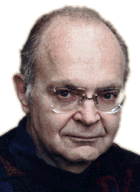
\includegraphics[width=.35\textwidth]{knuth}% A none-ps graphic
\hfill

\includegraphics[width=.60\textwidth]{elephant}%       A ps graphic

\subsection*{PSTricks code inside a pspicture environment}

\newpsobject{showgrid}{psgrid}{subgriddiv=1,griddots=10,gridlabels=8pt}

\begin{center}
\begin{pspicture}(-5.25,-5.25)(5.25,5.25)%
  \pscircle*[linecolor=Apricot]{5}
  \rput(0,0.5){
\includegraphics[width=8\psxunit]{elephant}}
  \Huge\sffamily\bfseries
  \rput(-4.5,4.5){A} \rput(4.5,4.5){B}
  \rput(-4.5,-4.5){C}\rput(4.5,-4.5){D}
  \rmfamily
  \rput(0,-3.8){PSTricks}
  \rput(0,3.8){\LaTeX}
  \showgrid
\end{pspicture}
\end{center}

\subsection*{PSTricks code without a pspicture environment}

%%----------------------------------------------------------------------
%% From: The \LaTeX\ Graphics Companion; first release.
\definecolor{pink}{rgb}{1, .75, .8}
\renewcommand\psedge{\nccurve}
\newcommand{\Female}[2][]{{\psset{linecolor=pink}\TR[#1]{\emph{#2}}}}
\newcommand{\Male}[2][]{{\psset{linecolor=blue}\TR[#1]{#2}}}
\psset{nodesep=2pt,angleA=90,angleB=-90}
\footnotesize 

\pstree[treemode=U]{\Female{{\bfseries Matilde}}}{%
  \pstree{\Male{Sebastian}}{%
    \pstree{\Male[name=P]{Philip}}{\Male{Frederick}\Female{Ethel}}
    \pstree{\Female[name=W]{Mary}}{\Male{Lionel}\Female{Agnes}}}
  \pstree{\Female{Leonor}}{%
    \pstree{\Male[name=R]{Ra\'ul}}{\Male{Joaquim}\Female{J\'ulia}}
    \pstree{\Female[name=A]{Am\'elia}}{\Male{\'Alvaro}\Female{Augusta}}}
}

%%----------------------------------------------------------------------

\subsection*{psfrag demo}

\normalsize

\noindent
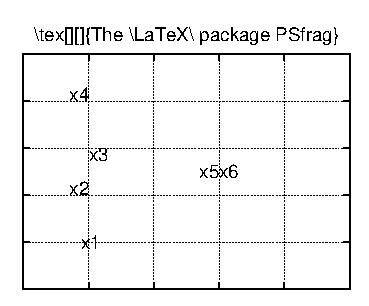
\includegraphics[width=.475\textwidth]{psf-demo.eps}
\hfill
\begin{psfrags}
  \psfragscanon
  \psfrag{x1}[br][  ]{\LaTeX} \psfrag{x2}[br][br]{\LaTeX}
  \psfrag{x3}[br][tl]{\LaTeX} \psfrag{x4}[br][Br]{\LaTeX}
  \psfrag{x5}[Br][ r][1.15][45]{\Huge\LaTeX}
  \psfrag{x6}[tl][ l][1.15][45]{\Huge\LaTeX}
  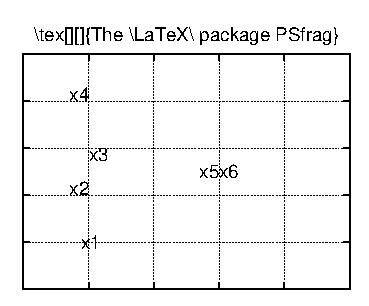
\includegraphics[width=.475\textwidth]{psf-demo}
\end{psfrags}

\subsection*{The postscript environment}

\begin{center}
\begin{postscript}
\Large
\noindent
$
  \bordermatrix{%
  & A            & B & C\cr
  & \rnode{D}{D} & E & \rnode{F}{F}\cr
  & G            & H & I\cr
  & \rnode{J}{J} & K & M
  }
$
\ncline[nodesep=-1em,linecolor=red]{D}{F}
\ncline[nodesep=-1em,linecolor=red]{D}{J}
\end{postscript}
\end{center}

\end{document}
%</example1>
%<*example2>
%% Process this file with the scripts `ps4pdf' or `ps4pdf.bat' or call
%%
%%   latex pst-pdf-example2.tex
%%   dvips -Ppdf -o pst-pdf-example2-pics.ps pst-pdf-example2.dvi
%%   ps2pdf -dAutoRotatePages=/None pst-pdf-example2-pics.ps pst-pdf-example2-pics.pdf
%%   pdflatex pst-pdf-example2.tex
%%
\listfiles\errorcontextlines=100\relax
\documentclass[12pt]{article}

%% before `psfrag'!
\usepackage[displaymath,dvipsnames]{pst-pdf}
%%\usepackage[displaymath,dvipsnames,notightpage]{pst-pdf}

\usepackage{pst-node,pst-tree}

\usepackage{psfrag,tabularx}

\pagestyle{empty}

\begin{postscript}[trim=0 0 0 0,ignore]
  
\includegraphics[width=.475\textwidth]{penguin.eps}
\end{postscript}
\savepicture{ps:A}


\begin{pst-pdf-defs}%

%% This definition must be within the pst-pdf-defs environment!
\newcommand*\mytree{%
  \begin{psmatrix}[rowsep=.2cm,colsep=2cm]
               &       & E   \\
               & A     &     \\
               &       & F   \\
  $\bullet$    &       &     \\
               &       & G   \\
               & B     &     \\
               &       & H   \\
  \scriptsize
  \psset{shortput=nab,arrows=->,labelsep=2pt,nodesep=2pt,nrot=:U}

  \ncline{4,1}{2,2}\ncput*{$0,2$}
  \ncline{4,1}{6,2}\ncput*{$x$}

  \ncline{2,2}{1,3}\ncput*{$0,3$}
  \ncline{2,2}{3,3}\ncput*{$y$}

  \ncline{6,2}{5,3}\ncput*{$z$}
  \ncline{6,2}{7,3}\ncput*{$0,8$}
  \end{psmatrix}%
}

\end{pst-pdf-defs}%

%% This works without the pst-pdf-defs environment!
\newcommand*\mymatrix{%
  \begin{postscript}
  \[
  \begin{array}{rcl}
   a & b & c \\
   1 & 2 & 3 \\
  \end{array}
  \]
  \end{postscript}%
}


\begin{document}

\setkeys{Gin}{showname,frame}%

\psset{unit=0.0714\textwidth}% 1/14 * \textwidth
\newpsobject{showgrid}{psgrid}{subgriddiv=1,griddots=10,gridlabels=6pt}

\newcommand*\BASEMARKER{\rule{.5em}{.4pt}}

\setlength\parindent{0pt}

\centering

\section*{\textsf{pst-pdf:}
  PSTricks and other PostScript code in pdf\LaTeX\ documents}

\vfill

\begin{pspicture}(-5.5,-5.25)(5.25,5.25)%
%%\begin{pspicture}[trim=-.5 -.25 .25 .25,frame](-5,-5)(5,5)% PSTricks2
  \pscircle*[linecolor=Apricot]{5}
  \rput(0,0.5){
\includegraphics[width=8\psxunit]{elephant}}
  \Huge\sffamily\bfseries
  \rput(-4.5,4.5){A} \rput(4.5,4.5){B}
  \rput(-4.5,-4.5){C}\rput(4.5,-4.5){D}
  \rmfamily
  \rput(0,-3.8){PSTricks}
  \rput(0,3.8){\LaTeX}
  \showgrid
\end{pspicture}\savepicture{ps:B}

\vfill\null\newpage

\usepicture{ps:A}
\hfill
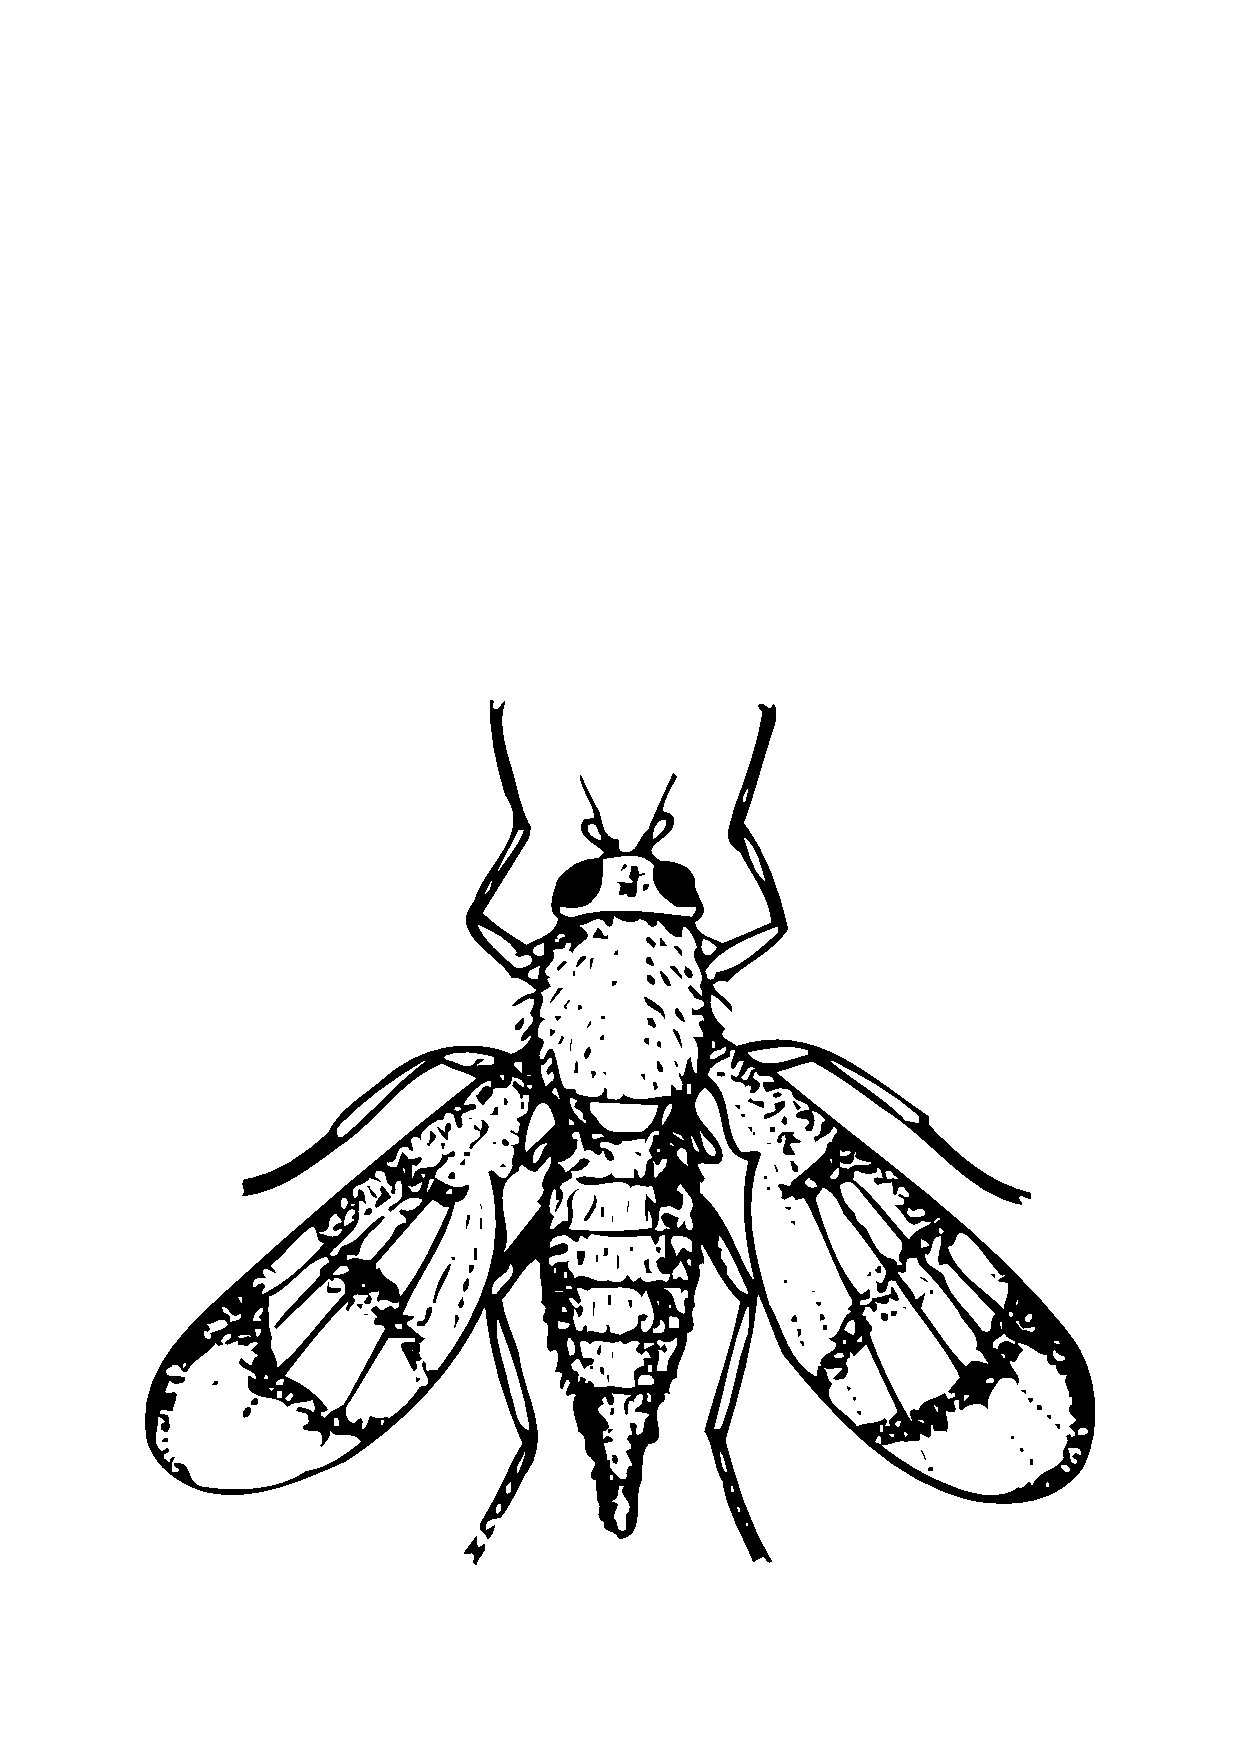
\includegraphics[width=.475\textwidth]{insect1}

\vfill

\usepicture[angle=180,origin=c]{ps:A}
\hfill
\usepicture[width=.47\textwidth]{ps:B}

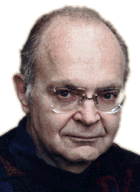
\includegraphics[width=.475\textwidth,frame=false,
  namefont={\Huge\itshape}]{knuth}
\hfill
\usepicture[angle=45,origin=bl,width=.475\textwidth,innerframe]{1}%

\vfill

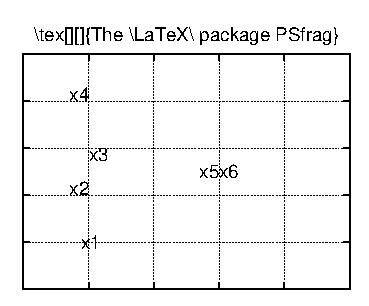
\includegraphics[width=.47\textwidth]{psf-demo}
\hfill
\begin{psfrags}
  \psfragscanon
  \psfrag{x1}[br][  ]{\LaTeX} \psfrag{x2}[br][br]{\LaTeX}
  \psfrag{x3}[br][tl]{\LaTeX} \psfrag{x4}[br][Br]{\LaTeX}
  \psfrag{x5}[Br][ r][1.15][45]{\Huge\LaTeX}
  \psfrag{x6}[tl][ l][1.15][45]{\Huge\LaTeX}
  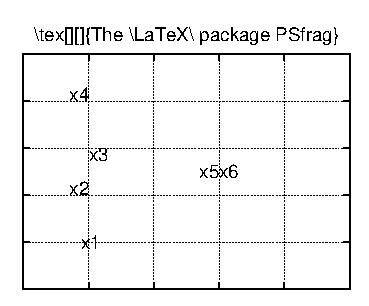
\includegraphics[width=.47\textwidth]{psf-demo}
\end{psfrags}

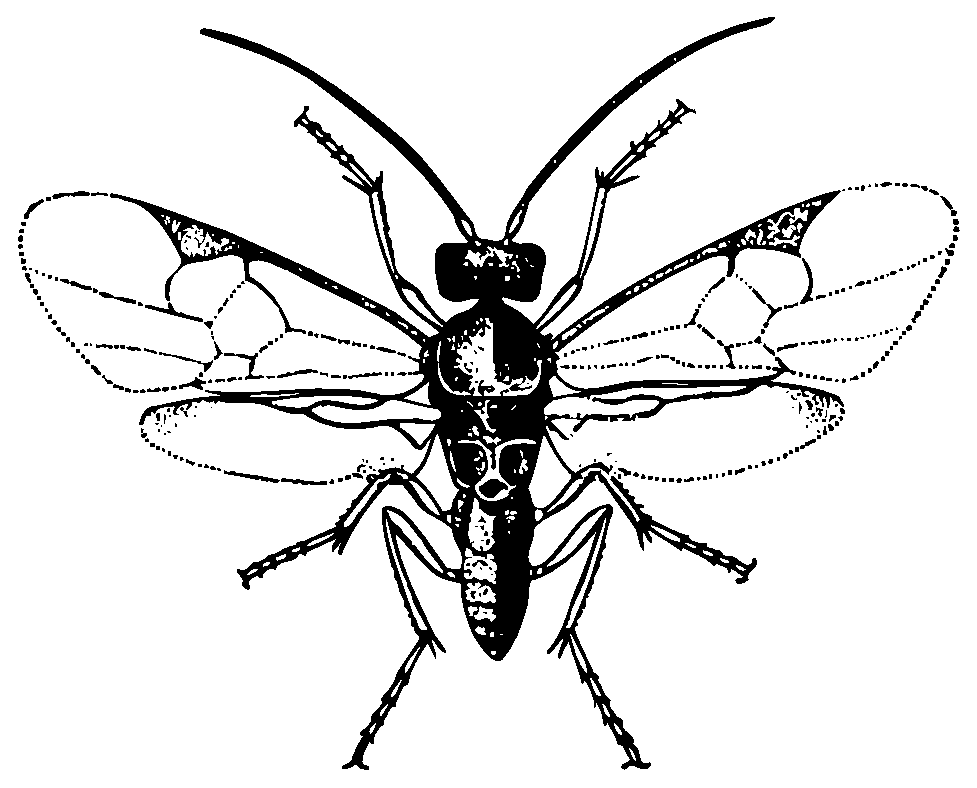
\includegraphics[width=\textwidth,showname=false,frame=false]{insect15}

\bigskip

\Large

\begin{equation}
  \sigma(t)=\frac{1}{\sqrt{2\pi}}
  \int^t_0 e^{-x^2/2} dx
\end{equation}

\clearpage

\setkeys{Gin}{showname=false,frame=false}%

{ \Huge \renewcommand*\arraystretch{1.5}

  \noindent
  \begin{tabularx}{\textwidth}{|@{}>{\centering}X@{}|} \hline

  \psframebox*[fillcolor=green,framearc=.6]{HUGO}\BASEMARKER
  \fbox{\BASEMARKER GUSTAV}  \tabularnewline

  \begin{postscript}
  \psframebox*[fillcolor=green,framearc=.6]{HUGO}\BASEMARKER
  \fbox{\BASEMARKER GUSTAV}
  \end{postscript}           \tabularnewline \hline

  \end{tabularx}

}

\bigskip

\definecolor{pink}{rgb}{1, .75, .8}
\renewcommand\psedge{\nccurve}
\newcommand{\Female}[2][]{{\psset{linecolor=pink}\TR[#1]{\emph{#2}}}}
\newcommand{\Male}[2][]{{\psset{linecolor=blue}\TR[#1]{#2}}}

\psset{nodesep=2pt,angleA=90,angleB=-90}

{ \footnotesize

   %% From: The \LaTeX\ Graphics Companion; first release.
   \pstree[treemode=U]{\Female{{\bfseries Matilde}}}{%
     \pstree{\Male{Sebastian}}{%
       \pstree{\Male[name=P]{Philip}}{\Male{Frederick}\Female{Ethel}}
       \pstree{\Female[name=W]{Mary}}{\Male{Lionel}\Female{Agnes}}}
     \pstree{\Female{Leonor}}{%
       \pstree{\Male[name=R]{Ra\'ul}}{\Male{Joaquim}\Female{J\'ulia}}
       \pstree{\Female[name=A]{Am\'elia}}{\Male{\'Alvaro}\Female{Augusta}}}
   }

  \iffalse  % --> Cannot work outside of a special environment!
  \psset{linecolor=green,doubleline=true,linestyle=dotted}
  \ncline{P}{W}\nbput{1940}
  \ncline{R}{A}\nbput{1954}
  \fi
}

\bigskip

\psset{arrows=->,fillcolor=white,fillstyle=solid}

\footnotesize

\newcommand{\Show}[1]{\psshadowbox{#1}}

\begin{psmatrix}[mnode=r,ref=t,unit=.3]
  \psframebox[linestyle=none,framesep=.75]{%
    \begin{psmatrix}[name=A,ref=c]
      \Show{Stakeholder}
    \end{psmatrix}} &
  \psframebox[fillstyle=solid,fillcolor=pink,framesep=.95]{%
    \rule{1cm}{0pt}
    \begin{psmatrix}[ref=c]
      [name=B]\Show{Goal} & \Show{Criteria}\\
              \Show{Sub-goal} & \Show{Justification}
      \ncline{1,1}{1,2}
      \ncline{1,1}{2,2}
      \ncline{1,1}{2,1}\tlput{Strategy}
      \ncline{2,1}{2,2}
    \end{psmatrix}}
  \ncline[angleB=180]{A}{B}\naput[npos=.7]{Model}
\end{psmatrix}

\begin{postscript}[angle=90,height=\textheight,frame=false]

\pstree[treemode=U]{\Female{{\bfseries Matilde}}}{%
  \pstree{\Male{Sebastian}}{%
    \pstree{\Male[name=P]{Philip}}{\Male{Frederick}\Female{Ethel}}
    \pstree{\Female[name=W]{Mary}}{\Male{Lionel}\Female{Agnes}}}
  \pstree{\Female{Leonor}}{
  \pstree{\Male[name=R]{Ra\'ul}}{\Male{Joaquim}\Female{J\'ulia}}
  \pstree{\Female[name=A]{Am\'elia}}{\Male{\'Alvaro}\Female{Augusta}}}
}

\psset{linecolor=green,doubleline=true,linestyle=dotted}
\ncline{P}{W}\nbput{1940}
\ncline{R}{A}\nbput{1954}

\end{postscript}

\bigskip

\psset{arrows=-}

\begin{displaymath}
  \bordermatrix{%
  & A            & B & C\cr
  & \rnode{D}{D} & E & \rnode{F}{F}\cr
  & G            & H & I\cr
  & \rnode{J}{J} & K & M
  }
  \ncline[nodesep=-1em,linecolor=red]{D}{F}
  \ncline[nodesep=-1em,linecolor=red]{D}{J}
\end{displaymath}

\bigskip

\mytree

\bigskip

\mymatrix

\end{document}
%</example2>
